\documentclass[a4paper,10pt, titlepage, twoside]{article}

\usepackage{graphicx, verbatimbox}
\usepackage[nottoc,numbib, section]{tocbibind}
\usepackage{braket}
\usepackage{amsmath}
\usepackage{amssymb}
\usepackage{wrapfig}
\usepackage[left=1in, right=1in]{geometry}
\usepackage{fancyhdr}
\usepackage[ddmmyyyy]{datetime}
\usepackage{float}
\usepackage{tikz}
\usepackage{subcaption}
\usepackage{hyperref}
\hypersetup{
    colorlinks=true,
    linktoc=all,
    linkcolor=blue,
}

\newcommand{\Mod}[1]{\ (\mathrm{mod}\ #1)}

\pagestyle{fancy}
\fancyhf{}
\fancyhead[LE, RO]{42807671 - psycjw}

\begin{document}
\begin{titlepage}
	\centering
	
\includegraphics{uonlogo}\par
	\vfill
	{\huge Christopher J. Wright \par}
	\vfill
	{\huge \textbf{ID:} 42807671\par}
	{\huge \textbf{Supervisor:} Prof. Thorsten Altenkirch\par}
	{\huge \textbf{Module:} G53IDS\par}
	\vfill
	{\huge 2018/19}
\end{titlepage}
\shipout\null
\thispagestyle{empty}
\begin{titlepage}
	\centering
	
\includegraphics{uonlogo}	
	\vfill
	{\scshape\large G53IDS Dissertation \par}
	{\scshape\LARGE Quantum Computing in Haskell \par}
	\vfill
	{\large Submitted April 2019, in partial fulfilment of the conditions for the award of the degree BSc Computer Science \par}
	\vfill
	{\large \textbf{Author:} 42807671, Christopher J Wright, psycjw \par}
	{\large \textbf{Supervisor:} Prof. Thorsten Altenkirch, psztxa \par}
	\vfill
	{\large School of Computer Science \par University of Nottingham}
	\vfill
	{I hereby declare that this dissertation is all my own work, except as indicated in the text.\par}
	\vfill
	\begin{flushleft}
		{\large \textbf{Signature} \par}
		\vfill
		{\large \textbf{Date} \hspace{2cm} \today\par}
	\end{flushleft}
\end{titlepage}
\shipout\null

\fancyhead[RE, LO]{ABSTRACT}
\section*{Abstract}
Quantum computing is growing daily as new quantum computers are created, and new research is done. There are already many desirable uses of quantum computing, such as factoring integers in $O(log N)$ \cite{shor} and searching unsorted databases in $O(\sqrt{N})$ \cite{grover}. There are even quantum games being created, such as Quantum Battleships \cite{qships}. \par
As the field expands, more people will find interest in the field and attempt to learn and pursue a career concerning quantum computers, and so suitable learning and experimental platforms need to be present to help this happen. This is the main inspiration for this project; create a stable up-to-date platform for users to run quantum computations on a classical computer via quantum simulation, while also improving my own understanding and experience of the subject for the future.\par
This dissertation explains the basics of quantum computing, and provides possible methods for the implementation of certain quantum algorithms on a classical computer using Haskell, with a quantum-computation simulating package called QIO \cite{qio}. This package already includes structures necessary for quantum computations, such as the qubit and unitary functions, however does not work on the latest Haskell update (v8.4.3) and lacks complex quantum algorithms. Therefore, the package is first updated, and then 2 quantum algorithms are implemented. Following this, a quantum circuit builder is designed and implemented in the package, allowing users to create and test quantum circuits using a intuitive GUI.\par
Each part of the project, namely the two algorithms implemented and the circuit builder, is completely separate and functions independantly, and so I split the project up into 3 parts. Each part is designed, implemented, tested and evaluated before moving to the next part - avoiding confusion between parts and ensuring one part is complete before attempting the next.
\newpage

\fancyhead[RE, LO]{\leftmark}
\tableofcontents
\clearpage
\fancyfoot[CE,CO]{\thepage}

\setcounter{page}{1}
\section{Introduction to Quantum Computing}
\subsection{Brief History}
The idea of a quantum computer was first introduced in a talk in 1981 by Nobel prize-winning physicist Richard P. Feynman. In his talk, reproduced in the \textit{International Journal of Theoretical Physics} in 1982 \cite{feynman}, he proposed that it would be impossible to simulate a quantum system on a classical computer efficiently. At the same time, physicist Paul Benioff demonstrated that quantum mechanical systems can model classical Turing machines \cite{benioff}, and created the first recognizable theoretical framework for a quantum computer. \par
This resulted in David Deutsch's creation of the first universal quantum computer \cite{deutsch}. This computer could do things that a universal Turing machine cannot, such as generate truly random numbers, and simulate finite physical systems. \par
Over time, quantum algorithms have been developed which solve problems faster and more efficiently than classical algorithms can, demonstrating the main use for quantum computers. The main examples of such algorithms would be the Deutsch-Jozsa algorithm  \cite{deutsch-jozsa}, Shor's algorithm \cite{shor} and Grover's algorithm \cite{grover}.

\subsection{QIO}
QIO is a Haskell package built by Alexander S. Green and Prof. Thorsten Altenkirch \cite{qio}, which allows users to simulate a quantum computer on their own classical computer. Typical quantum operations are built up of unitary (reversible) functions under a monoid \texttt{U}, and can then be run using a monad \texttt{QIO} and the function \texttt{applyU}. This \texttt{QIO} monad also has functions \texttt{mkQbit} and \texttt{measQbit}, which can be used to create a new qubit and measure an existing qubit respectively.\par
This leads to an intuitive platform which can be used to create quantum computations, and then run/simulate them with 2 very simple functions \texttt{run :: QIO a -> IO a}  and \texttt{sim :: QIO a -> Prob a}, where \texttt{run} is used to execute a quantum computation and return the value of qubits measured based on their probabilities and a pseudorandom number generator. The \texttt{sim} function is similar, however after executing a quantum computation, it returns the probability distribution for the qubits measured, showing the possible states and their probabilities when measured.\par
I will use this package to help introduce and teach quantum computing, providing relevent code segments to improve clarity, and create programs to highlight certain features of quantum computations.

\subsection{The Qubit}
A classical computer uses a bit to store data. This bit can only be in one of two states, 0 or 1. Strings of bits are then used to represent data and instructions, forming the basis of classical computation.\par
However, a quantum computer uses a quantum bit, known as a qubit. This qubit can simply be in the classical states 0 or 1, or in a superposition of both, i.e., be in both states at once. This means an operation performed on a qubit effectively acts on both 0 and 1 at the same time.\par
A qubit can be described by a linear combination of $\ket{0}$ and $\ket{1}$, 
$$\ket{\psi}=\alpha\ket{0} + \beta\ket{1},\quad \alpha,\beta \in \mathbb{C},\quad |\alpha^2| + |\beta^2| = 1$$
where $ |\alpha^2|$ represents the probability of measuring the $0$ state, and $|\beta^2|$ the $1$ state. Hence the normalization condition $|\alpha^2| + |\beta^2| = 1$. This condition also corresponds to the fact that $\ket{\psi}$ is a unit vector in the complex vector space.\par
Measuring a qubit will collapse its wave function due to Born's rule \cite{born}. This means that, when measured, a qubit will collapse to be either $\ket{0}$ or $\ket{1}$. For example, if we take the qubit
$$\ket{+} = \frac{1}{\sqrt{2}}\ket{0} + \frac{1}{\sqrt{2}}\ket{1}$$
and measure it, the probability of getting $\ket{0}$ or $\ket{1}$ is $\frac{1}{2}$. We can therefore say that the qubit $\ket{+}$ is in an equal superposition.\par
In QIO, a qubit is referred to as a \texttt{Qbit}. One can be created simply using the \texttt{mkQbit :: Bool -> QIO Qbit} function mentioned above, and is created based on the boolean value passed in. The function \texttt{measQbit :: Qbit -> QIO Bool} can then later be used to measure the state of the qubit passed in.
\begin{verbatim}
make2qubits :: QIO (Bool, Bool)
make2qubits = do
    q0 <- mkQbit False -- This will create a qubit, q0, in the state |0>
    q1 <- mkQbit True -- This will create a qubit, q1, in the state |1>
    b0 <- measQbit q0 -- This will measure the qubit q0, returning False
    b1 <- measQbit q1 -- This will measure the qubit q1, returning True
    return (b0, b1) -- Returns (False, True)
\end{verbatim}
Qubit base states can also be represented as vectors, with $\ket{0} = 
\begin{bmatrix}
	1 \\ 0
\end{bmatrix}$
and $\ket{1} = 
\begin{bmatrix}
	0 \\ 1
\end{bmatrix}$.
The qubit $\ket{\psi}$ above can be rewritten, introducing a multiplier known as the global phase, making the coefficient for $\ket{0}$ (i.e., $\alpha$) real and non-negative. For example, the state $\frac{-i}{\sqrt{2}}\ket{0} + \frac{i}{\sqrt{2}}\ket{1}$ is the same as  $\frac{1}{\sqrt{2}}\ket{0} + \frac{-1}{\sqrt{2}}\ket{1}$ with a global phase of $-i$. This global phase does not affect the amplitudes of the states, and so doesn't change the qubit's value when measured.\par
This qubit state $\ket{\psi}=\alpha'\ket{0} + \beta'\ket{1}$  can now be written in the form
$$\ket{\psi} = \cos(\frac{\theta}{2})\ket{0} + e^{i\phi}\sin(\frac{\theta}{2})\ket{1},\qquad \theta = 2\cos^{-1}(\alpha'), \quad \phi = \Im(\ln(\frac{\beta'}{\sin(\frac{\theta}{2})}),$$
$$0 \leq \theta \leq \pi,\quad 0 \leq \phi \leq 2\pi$$
From this, it is easy to see that a qubit can be represented geometrically using the angles $\theta$ and $\phi$, on what is known as the Bloch sphere.

\subsection{The Bloch Sphere}
The Bloch sphere, named after physicist Felix Bloch, is a geometrical representation of a two-state quantum mechanical system (e.g. a qubit). As shown above, a qubit's coefficients can be expressed in terms of 2 angles, $\theta$ and $\phi$. This makes it extremely easy to see what happens when operations are performed on qubits, and it is clear that a qubit pointing to a point above the origin has a higher $\ket{0}$ amplitude than $\ket{1}$, and vice versa.\par
\begin{figure}[H]
	\centering
	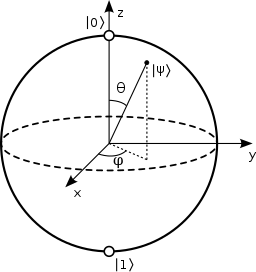
\includegraphics[width=0.25\textwidth]{blochsphere}
	\caption{A Qubit represented geometrically on the Bloch Sphere}
\end{figure}
We can calculate the angle $\theta$ using QIO's underlying structure and the \texttt{sim} function. The angle $\phi$ cannot be calculated in this way, as we use the probabilities for each state for the calculation.\par
The \texttt{sim} function returns a value of type \texttt{Prob a}, where \texttt{a} is given by the quantum computation it is applied to (i.e. applying \texttt{sim} to a function of type \texttt{QIO Bool}, will return a value of type \texttt{Prob Bool}). This \texttt{Prob} type is simply a wrapper around vectors given by real probabilities, defined in the \texttt{Qio.hs} file:
\begin{verbatim}
data Prob a = Prob {unProb :: Vec RR a}
\end{verbatim}
where \texttt{RR} is simply a \texttt{Double} value, and \texttt{Vec} is a wrapper around a list of pairs, defined in the \texttt{Vec.hs} file:
\begin{verbatim}
newtype Vec x a = Vec {unVec :: [(a,x)]} deriving Show
\end{verbatim}
From this, it is easy to see that
\begin{verbatim}
Prob Bool = Prob {unProb :: Vec RR Bool} 
          = Prob {unProb :: Vec {unVec :: [(Bool, Double)]}}
\end{verbatim}
Now, we can extract the probabilities for qubits, and calculate $\theta$.
\begin{verbatim}
quantum :: QIO Bool
quantum = do
    q <- mkQbit True
    measQbit q
    
theta :: QIO Bool -> Double
theta c = 2 * (acos alpha)
    where
        ps = unVec $ unProb $ sim c
        alpha = sqrt $ snd $ last ps
\end{verbatim}
The function \texttt{quantum} can be changed to perform any operation on the qubit, and as long as the function's type does not change, then \texttt{theta quantum} will always return $\theta$ for the qubit measured. E.g.
\begin{verbatim}
quantum :: QIO Bool        -> theta quantum = 3.141592653589793
quantum = do
    q <- mkQbit True
    measQbit q

quantum :: QIO Bool        -> theta quantum = 0.0
quantum = do
    q <- mkQbit False
    measQbit q

quantum :: QIO Bool        -> theta quantum = 1.5707963267948966
quantum = do
    q <- mkQbit False
    applyU (uhad q)
    measQbit q
\end{verbatim}

\subsection{Decoherence}
Put simply, decoherence is the loss of coherence. This basically means that the quantum state described by a system is no longer in superposition, and leads to a collapse of the wave function. If this occurs during a computation, all information stored in qubits is lost, and the computation needs to be restarted. Decoherence can occur naturally after a certain amount of time as the system will be entangled with its environment \cite{decoherence}, and is the main problem quantum computing faces.

\subsection{Basic Operations}
\subsubsection{1-Qubit Gates}
A 1-qubit gate can be thought of as a rotation about the Bloch sphere, and as the state space of a qubit is continuous, there are an infinite amount of 1-qubit gates. Any complex unitary 2x2 matrix represents a 1-qubit gate, and there are 4 main 1-qubit gates: the Hadamard gate, and the 3 Pauli- gates. Note that all quantum gates must be unitary (i.e., is its own inverse).\par
As mentioned earlier in section 1.2, QIO uses a monoid \texttt{U} to form unitary functions. These functions are defined as 5 distinct forms, using recursion to create sequences of functions:
\begin{verbatim}
data U = UReturn
       | Rot Qbit Rotation U
       | Swap Qbit Qbit U
       | Cond Qbit (Bool -> U) U
       | Ulet Bool (Qbit -> U) U
\end{verbatim}
\texttt{UReturn} is simply an empty function, and will always be the last unitary in a sequence. For this section on 1-Qubit gates, the \texttt{Rot Qbit Rotation U} form is used. QIO defines all single qubit gates as rotations, where a \texttt{Rotation :: ((Bool, Bool) -> CC)} represents the 2x2 matrix of the gate. The \texttt{rot} function is then used to create a unitary function for a given \texttt{Rotation} and qubit.
\begin{verbatim}
rot :: Qbit -> Rotation -> U
rot x r = Rot x r UReturn
\end{verbatim}

\paragraph{The Hadamard Gate}
Named after French mathematician Jacques Hadamard, the Hadamard gate (also called the Hadamard rotation) takes the base states $\ket{0}$ and $\ket{1}$ into equal superpositions
$$\ket{0} \mapsto \frac{1}{\sqrt{2}}(\ket{0} + \ket{1}) = \ket{+}$$
$$\ket{1} \mapsto \frac{1}{\sqrt{2}}(\ket{0} - \ket{1}) = \ket{-}$$
and has the matrix $\frac{1}{\sqrt{2}} 
\begin{bmatrix}
	1 & 1 \\
	1 & -1 
\end{bmatrix} $.
It is equivalent to the combination of 2 rotations: $\pi$ about the Z-axis, followed by $\pi/2$ about the Y-axis.
\begin{figure}[H]
	\centering
	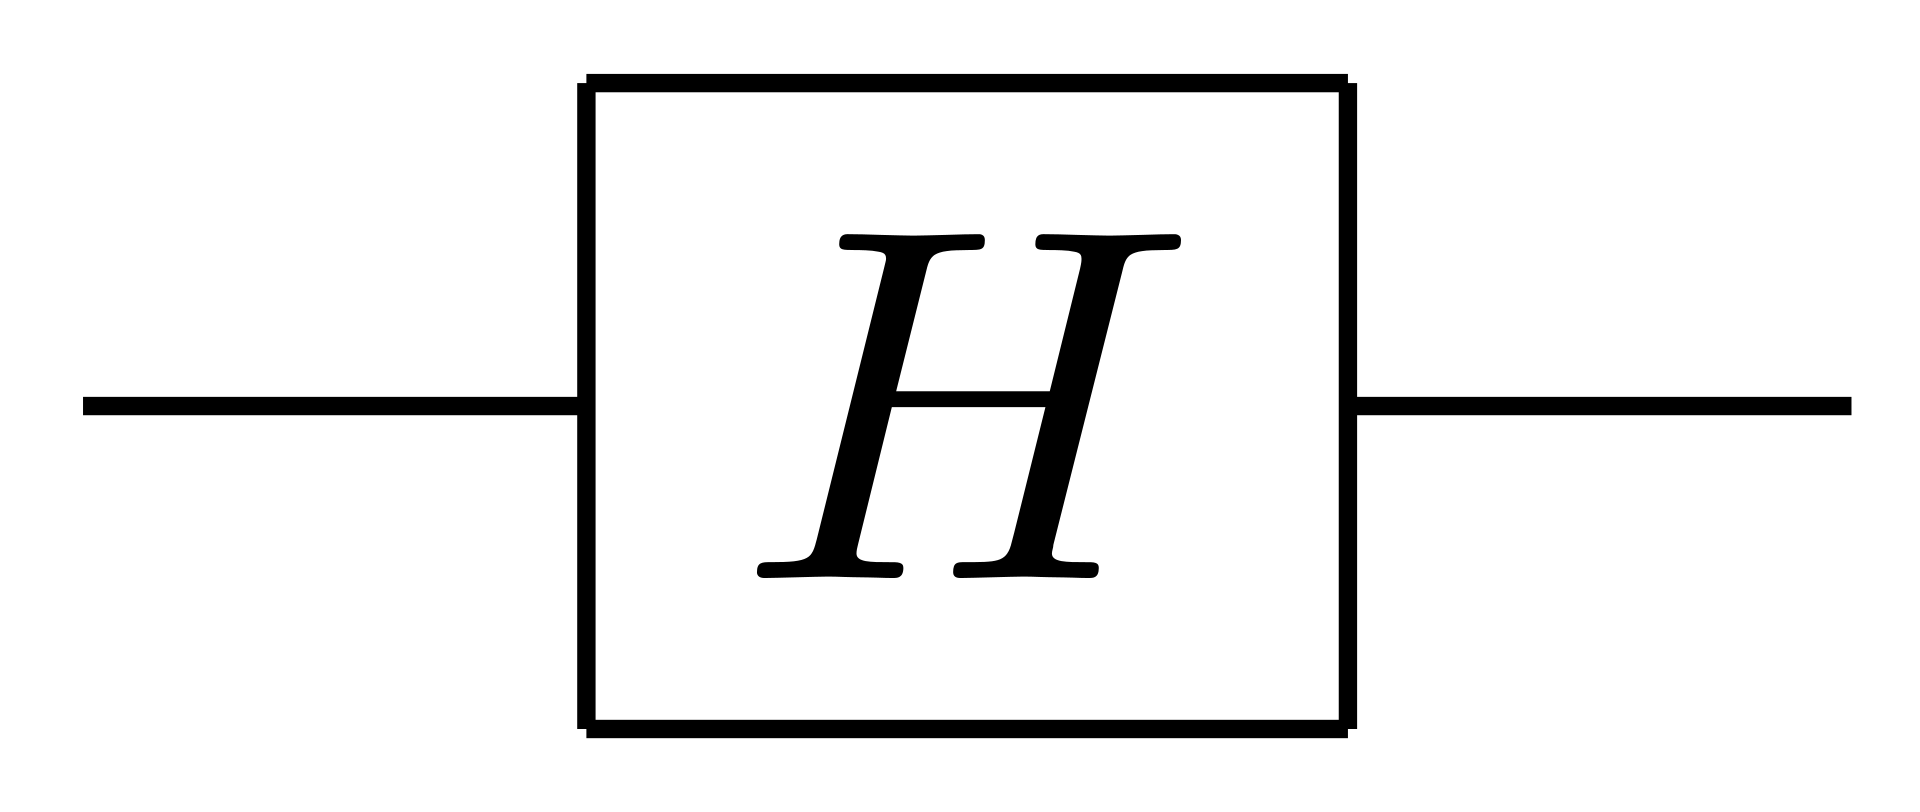
\includegraphics[width=0.25\textwidth]{hadamard}
	\caption{The Hadamard Gate}
\end{figure}
The gate matrix (i.e. \texttt{Rotation}) is given by \texttt{rhad} in the \texttt{QioSyn.hs} file, along with the unitary function \texttt{uhad} which can be used via the \texttt{applyU} function.
\begin{verbatim}
rhad :: Rotation
rhad (x,y) = if x && y then -h else h where h = (1/sqrt 2)

uhad :: Qbit -> U
uhad x = rot x rhad

applyHadamard :: QIO Bool
applyHadamard = do
    q <- mkQbit False
    applyU (uhad q)
    measQbit q
\end{verbatim}

\paragraph{The Pauli- Gates}
The Pauli- gates, created by Wolfgang Pauli, correspond to a rotation of $\pi$ about one of the 3 axis, and so there are 3 - Pauli-X, Pauli-Y and Pauli-Z (often abbreviated to X, Y and Z respectively). The Pauli-X gate is most common, as it is the equivalent of a classical NOT gate.

$$
X = 
\begin{bmatrix}
	0 & 1 \\
	1 & 0
\end{bmatrix},
\quad Y =
\begin{bmatrix}
	0 & -i \\
	i & 0
\end{bmatrix},
\quad Z =
\begin{bmatrix}
	1 & 0 \\
	0 & -1
\end{bmatrix}$$
\begin{figure}[H]
	\centering
	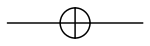
\includegraphics[width=0.25\textwidth]{not}
	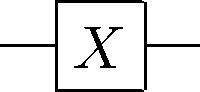
\includegraphics[width=0.18\textwidth]{paulix}
	\caption{The 2 representations of the Pauli-X (NOT) Gate}
\end{figure}
The Pauli-X gate is defined in QIO using the \texttt{rnot Rotation} and the unitary \texttt{unot}. However, these gates can be created simply by first creating the corresponding \texttt{Rotation} matrix, and then using the \texttt{rot} function similar to how the Hadamard gate is defined.

\begin{verbatim}
rX :: Rotation                          uX :: Qbit -> U
rX (x,y) = if x==y then 0 else 1        uX q = rot q rX

rY :: Rotation                          uY :: Qbit -> U
rY (False, True) = 0 :+ 1               uY q = rot q rY
rY (True, False) = 0 :+ (-1)
rY (_, _) = 0

rZ :: Rotation                          uZ :: Qbit -> U
rZ (False, False) = 1                   uZ q = rot q rZ
rZ (True, True) = -1
rZ (_, _) = 0
\end{verbatim}

\subsubsection{n-Qubit Gates}
Alongside the gates above, there are 3 other basic quantum gates; Controlled-X, SWAP and Toffoli, which are defined in QIO using the other 3 constructs for \texttt{U}.

\paragraph{The SWAP Gate}
This gate is extremely simply; it just swaps 2 qubits. In QIO, it is defined by the \texttt{swap} function.
\begin{verbatim}
swap :: Qbit -> Qbit -> U
swap x y = Swap x y UReturn
\end{verbatim}

\paragraph{The Controlled-X Gate}
The most common 2-qubit gate, it applies the Pauli-X gate (i.e., a NOT gate) on the second qubit if and only if the first qubit is $\ket{1}$. It is often called the Controlled-NOT or cNOT gate. Note that we can do the same with the other Pauli- gates, however this is rarely used.\par
The gate is defined using the \texttt{Cond Qbit (Bool -> U) U} unitary construct, and the function \texttt{cond} which creates the unitary (similar to the functions \texttt{rot} and \texttt{swap} above). Essentially, when given a qubit and a unitary function which takes in a boolean, the resulting unitary will apply the boolean function to the states the qubit can be in.\par
This is best demonstrated with an implementation for the cNOT gate. If the qubit is measured to be \texttt{True} (i.e. in the $\ket{1}$ state), then the resulting unitary is a NOT gate. Otherwise, nothing will be done and the resulting unitary is empty.
\begin{verbatim}
cond :: Qbit -> (Bool -> U) -> U
cond x br = Cond x br UReturn

cnot :: Qbit -> Qbit -> U
cnot qc qo = cond qc (\x -> if x then (unot qo) else mempty)
\end{verbatim}

\paragraph{The Toffoli Gate}
This gate acts on 3 qubits, and is often called the ccNOT gate. This is because it applies the Pauli-X gate on the third qubit if and only if the first two qubits are both $\ket{1}$. 
\begin{verbatim}
toffoli :: Qbit -> Qbit -> Qbit -> U
toffoli q1 q2 qo = cond q1 (\x -> if x then (cnot q2 qo) else mempty)
\end{verbatim}
\begin{figure}[H]
	\centering
	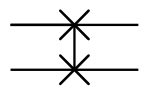
\includegraphics[width=0.25\textwidth]{swap}
	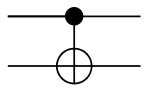
\includegraphics[width=0.25\textwidth]{cnot}
	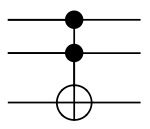
\includegraphics[width=0.25\textwidth]{toffoli}
	\caption{The SWAP gate (left), the Controlled-X (cNOT) gate (middle), and the Toffoli gate (right)}
\end{figure}

\paragraph{The $C^n$-NOT Gate}
The idea behind the Toffoli gate above (multiple control qubits, and one output qubit) can be extended to any arbitrary amount, creating a $c^n$-NOT gate. From the definition of the Toffoli gate in QIO above, it is clear that we can define a gate in QIO which acts on a list of control qubits, and one output qubit.
\begin{verbatim}
cNnot :: [Qbit] -> U
cNnot [] = mempty
cNnot (q:qs) = cond q (\x -> if x then (cNnot qs) else mempty)
\end{verbatim}
However, this only works due to how QIO operates on qubits. On a quantum computer, a gate like this will require a sequence of toffoli gates and ancilla qubits. For example, the cccNOT gate requires an extra ancilla qubit:
\begin{verbatim}
cccNot :: Qbit -> Qbit -> Qbit -> Qbit -> Qbit -> U
cccNot q1 q2 q3 q4 qa = 
    toffoli q1 q2 qa <>
    toffoli q3 qa q4 <>
    toffoli q1 q2 qa
\end{verbatim}
\begin{figure}[H]
	\centering
	\theverbbox\qquad
	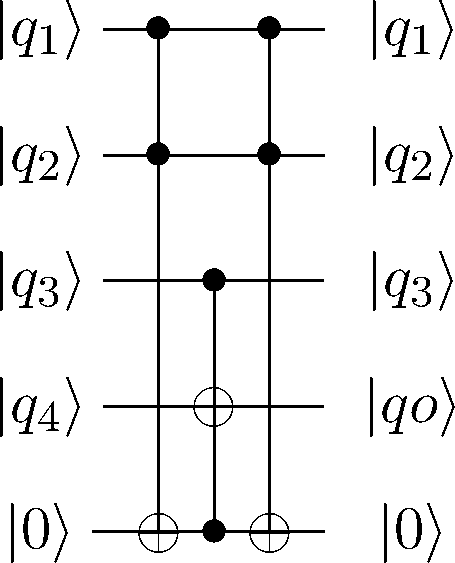
\includegraphics[width=0.25\textwidth]{cccnot}
	\caption{The cccNOT gate, made using toffoli gates and an ancilla qubit, where $\ket{qo} = \ket{q_4 \oplus (q_1 q_2 q_3)}$}
\end{figure}
When using ancilla qubits in QIO, we can use the unitary construct \texttt{Ulet} and the function \texttt{ulet}.
\begin{verbatim}
ulet :: Bool -> (Qbit -> U) -> U
ulet b ux = Ulet b ux UReturn
\end{verbatim}
This construct will create a qubit in the state given by the boolean, for use in the given unitary. We can now execute the cccNot gate defined above. The qubit \texttt{q4} will be set to $\ket{1}$ if and only if \texttt{q1, q2} and \texttt{q3} are all in the state $\ket{1}$.
\begin{verbatim}
doCccNOT :: QIO Bool
doCccNOT = do
    q1 <- mkQbit True
    q2 <- mkQbit True
    q3 <- mkQbit True
    q4 <- mkQbit False
    applyU (ulet False (cccNot q1 q2 q3 q4))
    measQbit q4
\end{verbatim}

\subsection{Entanglement}
Quantum entanglement is a phenomenon that occurs when the value of one qubit affects another, and forms a large part of many quantum algorithms. As mentioned above, when we measure a qubit it collapses to one of its base states. If another qubit depends on this measured qubit (e.g., via a cNOT gate), then it will also collapse to one of the base states. The 2 qubits are then said to be entangled. \par
Consider a circuit which starts with two qubits \textit{Alice} and \textit{Bob}, both starting in the state $\ket{0}$. We then apply the Hadamard gate to \textit{Alice}, converting \textit{Alice} into an equal superpositional state of the base states $\ket{+} = \frac{1}{\sqrt{2}}(\ket{0} + \ket{1})$, meaning there is a 50/50 chance of \textit{Alice} being 0/1 when measured. Next, we apply a cNOT gate to \textit{Alice} and \textit{Bob}, entangling the two qubits together. Therefore, if we measure \textit{Alice} to be $\ket{0}$, then \textit{Bob} will collapse to the state $\ket{0}$, and the same will occur for the state $\ket{1}$. As entanglement is non-local, \textit{Alice} and \textit{Bob} could be separated by any distance, and this will still occur.\par
This can be implemented in QIO using the \texttt{uhad} and \texttt{cnot} defined earlier. The function \texttt{entangle} below will create 2 qubits, \texttt{qa} and \texttt{qb}, and initialize them in the $\ket{0}$ state. We then apply the Hadamard gate to qa, changing its state to $\frac{1}{\sqrt{2}}(\ket{0} + \ket{1})$ and a controlled-X unitary function, concatenated simply with the mappend operator \texttt{<>}. When run using the \texttt{run} function, \texttt{[True, True]} or \texttt{[False, False]} will be returned due to the entanglement. The \texttt{sim} function will return \texttt{([True, True], 0.5), ([False, False], 0.5)}.\par
\begin{verbatim}
entangle :: QIO [Bool]
entangle = do
    qa <- mkQbit False
    qb <- mkQbit False
    applyU (uhad qa <> cnot qa qb)
    ba <- measQbit qa
    bb <- measQbit qb
    return [ba, bb]
\end{verbatim}

\subsection{The Bell States}
The two qubits shown above, \textit{Alice} and \textit{Bob}, together form a Bell state, named after physicist John S. Bell
$$\ket{\Psi_{00}} = \frac{1}{\sqrt{2}}\ket{00} + \frac{1}{\sqrt{2}}\ket{11} = \frac{1}{\sqrt{2}}(\ket{00} + \ket{11})$$
As evident from the equation, if one of the qubits is measured to be $\ket{0}$ or $\ket{1}$, then so is the other. There are 4 Bell states, where each state has 2 entangled qubits, and the measurement of one qubit collapses the state of the other.
$$\ket{\Psi_{00}} = \frac{1}{\sqrt{2}}(\ket{00} + \ket{11}) \quad \ket{\Psi_{01}} = \frac{1}{\sqrt{2}}(\ket{01} + \ket{10})$$
$$\ket{\Psi_{10}} = \frac{1}{\sqrt{2}}(\ket{00} - \ket{11}) \quad \ket{\Psi_{11}} = \frac{1}{\sqrt{2}}(\ket{01} - \ket{10})$$
Each Bell state is created using the same unitary operation, namely a Hadamard gate on the first qubit, and then a cNOT to the second qubit using the first qubit as the control bit, with the resulting Bell state determined by the original state of the 2 qubits.

\section{Motivations}
\subsection{Problems}
A quantum computer consists of multiple two-level quantum-mechanical systems, such as multiple electrons, with each electron represents a qubit. The spin of the electron determines the qubit state, with spin up representing $\ket{0}$ and spin down representing $\ket{1}$. The main problem faced here is decoherence \cite{decoherence2}. The overall system is extremely sensitive to interaction with the surroundings, such as magnetic fields affecting electrons, and must be isolated from its environment. The more qubits we have, the harder it is to maintain coherence.\par
Due to the difficulties of creating a quantum computer, we need to be able to simulate one on a classical computer. This simulation will not be as efficient as a quantum computer, and so its main use is the testing and creation of quantum algorithms, alongside teaching quantum computing. This means there is a high demand in quantum computing simulators, hence the need for projects like this.

\subsection{Simulators}
As mentioned above, creating a stable and effective quantum computer is difficult, and so while new ways of implementation are being researched, we can use quantum simulators to create, test and teach quantum computing. As quantum computing grows even larger, simulators need to be available to people in order to help them learn about quantum computations and programs. More quantum simulators across different programming languages will supply a wider range of programmers the ability to practice quantum computing on their own computer, as well as offer different methods of implementing a quantum simulator.\par
This project aims to add to this group of quantum simulators, offering an up-to-date and reliable Haskell package which enables users to create and run quantum programs. On top of this, they will be able to run quantum algorithms over their own data sets, increasing the teaching ability of the project.

\section{Related Work}
\subsection{IBM Q}
The IBM Q Experience is an online platform \cite{ibmqexperience} - found easily with a Google search "ibm q" - which gives its users access to a set of prototype quantum processors. Users can create quantum circuits or programs via a graphical or textual interface, and then either run these quantum operations on an actual quantum computer, or simulate them classically.\par
It was launched by IBM in 2016 \cite{ibmlaunch}, and started with a 5 qubit quantum processor and matching simulator, alongside a small set of two-qubit operations. Over time, the platform has evolved into a strong stable quantum platform, with the addition of more 2-qubit operations, a simulator over a maximum of 20 qubits and limited beta access to a 16 qubit quantum processor. IBM also released a python-based quantum computing framework, QISKit \cite{qiskit}, allowing users to simulate a quantum computer offline, or run quantum programs on the real IBM quantum processors online.

\subsubsection{Evaluation}
In my opinion, the IBM Q Experience platform is great for all who wish to create quantum programs and just generally experiment with quantum computing. A colourful, intuitive graphical interface can be used to build quantum circuits and then run/simulated with ease - perfect for new users. This still works well for more advanced users, however the textual interface is more suited for advanced use. Complex quantum programs can be created instead of circuits, and the use of the QISKit framework enables users the option of creating and simulating quantum computations without the online platform. However, this does mean users must learn a new programming language, potentially alongside learning about quantum computations, creating quite a large knowledge gap to bridge. Yet this is somewhat diminished by the availability of two user guides, a Beginner's guide \cite{ibmqbeginner} and a Full guide \cite{ibmqfull}.\par
These guides successfully reduce the difficulty in learning the basics of quantum computing without confusing newcomers. The Beginner's guide briefly explains the qubit, and common single qubit gates. It then goes on to hint at some multi qubit gates, and explain the process of entanglement and how it can be used. The Full guide extends these sections, providing a greater depth of knowledge concerning the qubit, such as the Bloch sphere and decoherence, while going into more detail on single and multi qubit gates, with descriptions of quantum algorithms and some quantum error correction methods. More help is then available to users via a community forum \cite{ibmqforum} and in-depth QISKit tutorials \cite{ibmqiskit}, ensuring users can find solutions to any problems they are having.

\subsubsection{Key Points}
\begin{enumerate}
	\item Simple and effective graphical user interface, allowing the user to drag-and-drop quantum gates onto a circuit, with bright colours used to emphasize different gates.
	\item Basic textual interface, providing users with an interface they can use to build more complex quantum programs.
	\item Multiple user guides to help teach newcomers without confusing them, while still providing aid to more advanced users. 
	\item Emphasis placed on usability.
\end{enumerate}

\section{Project Description}
\subsection{Aim}
The aim of this project is to update and improve an out-of-date Quantum computing package in Haskell, QIO \cite{qio} - developed by Green and Altenkirch. This will result in an updated, stable package for Haskell v8.4.3, allowing users to simulate a quantum computer, and run various quantum algorithms. It will also provide the user a graphical interface to build and run quantum circuits. \par
This QIO Haskell package allows a user to create a quantum program, and then run or simulate it. By running, any qubits measured via a function \texttt{measQbit :: Qbit -> QIO Bool} will be collapsed into True or False based on their probability amplitudes and a pseudorandom number generator. However, the difference between this package and others is revealed when we simulate the program instead. Then, any qubits measured will be shown as their probabilities, including multiple qubits together. From this we can easily check the program for errors.\par
The package is currently not working in Haskell v8.4.3, and so first needs to be updated. The update will need to maintain the quantum aspects necessary for quantum computation, such as coherence and the no-cloning theorem, and still be able to run/simulate quantum programs inputted. \par
Following this, two quantum algorithms (Grover's and Shor's) will be implemented in the package, allowing users to run these algorithms on their own data. There is already an implementation of Shor's algorithm present in QIO, but this needs to be updated. Each implementation will be in a separate Haskell file, and be able to perform a quantum algorithm correctly over its inputs using the rest of the QIO package.\par
Finally, a quantum circuit builder/interpreter will be built. It will display a graphical interface, and allow the user to drag-and-drop quantum gates onto a circuit of any amount of qubits. It will then display the resulting amplitude(s) and/or value(s) of any of the qubits. This will be similar to the IBM Q Program specified above, only shall be run on a classical computer instead of a quantum one.

\subsection{Algorithms}
\subsubsection{Grover's algorithm}
In 1996, Lov K. Grover demonstrated an algorithm which could search a quantum mechanical database quickly \cite{grover}. This quantum algorithm is quadratically faster than the fastest classical variant, returning the index of the search item in $O(\sqrt{n})$, instead of the classical $O(n)$. It can also be generalized to find solutions to an unknown predicate function $f$ in the same time. This means that any problem which involves finding solutions to a boolean function can be solved using Grover's algorithm, and so it has a large variety of uses past searching databases, such as finding the mean and median of a set of numbers, or solving the collision problem in $O(n^{1/3})$\cite{collision} instead of the classical $\Theta (\sqrt n)$\par
The algorithm takes a function $f$, and after converting it into a unitary function, runs it over a set of qubits representing the data set to search. It then negates solution states in the solution set, and disperses them. This dispersion acts as an inversion around the mean amplitude, meaning the solution state is amplified due to the previous negation. After repeating this a number of times no greater than $\pi/4\sqrt{N}$ times, where $N$ is the amount of variables in the function, there is a high probability that the qubits, when measured, will give a solution to the function $f$.\par
This project aims to explore potential methods of implementating this algorithm in the QIO Haskell package, as well as demonstrate other ways of executing the algorithm.

\subsubsection{Shor's algorithm}
Before Grover's algorithm, there was Shor's algorithm for integer factorization. This quantum algorithm is used to find the factors of any integer $N$ in ~$O((log N)^3)$ \cite{shorcomplexity}. The algorithm specifically looks at the case of factorizing an integer $N = pq$, where $p$ and $q$ are both large primes. If an integer $b$ shares no factors with $N$ then $b^r = 1 \Mod N$ for some integer $r$, and the function $f(x) = b^x \Mod N$ is a periodic function of $x$ with period $r$. With the period $r$ known, if it is even we can calculate
$$x = b^{\frac{r}{2}} \Mod N$$
Following this, if $x + 1 \neq 0 \Mod N$ we can factorize the input. The probability of choosing a random $b$ which gives a period $r$ with these properties is $>50\%$ \cite{nsc}\textsuperscript{Shor's algorithm continued, page 27}.\par
After constructing a unitary function $U_{f(x)} = b^x \Mod N$, the algorithm applies it over an input state, leaving an equal superpositional state 
$$\frac{1}{\sqrt{2^n/2}}\sum_{x=0}^{2^n-1} \ket{x}_n \ket{b^x \Mod N}_{n_0}$$
$$n_0 =\log_2 N,\quad n = 2n_0$$
We can then measure the second register, which will give any value for $b^x mod N$, leaving the first register in an equal superposition over the values for $x$. The algorithm then applies the Quantum Fourier Transformation (QFT) to the first register and measures it, giving a value for $y$ where $y = 2^n/r$. Finally, we can check if $r$ is even and if $x + 1 \neq 0 \Mod N$ where $x = b^{r/2} \Mod N$, and if they are both true, then $N$ has factors $(x-1)$ and $(x+1)$. We can then find the greatest common denominators of both in $N$, corresponding to the 2 prime factors of $N$.

\section{The QIO Package}
\subsection{Underlying Structure}
QIO currently uses a HeapMap to store the states of the qubits in the system, and a Qbit type which just acts as an integer reference to this map. Unitary functions take the form of a monoid \texttt{Unitary}, and represent an operation on the HeapMap which may produce a new state. We can then restrict unitary functions to be in a few distinct forms, ensuring the functions are indeed unitary - a necessity for quantum computations. These forms are defined in a datatype \texttt{U} shown below.
\begin{verbatim}
data U = UReturn 
       | Rot Qbit Rotation U 
       | Swap Qbit Qbit U 
       | Cond Qbit (Bool -> U) U 
       | Ulet Bool (Qbit -> U) U
\end{verbatim}

Using recursion, this type dictates is what a unitary operation will be; a string of rotations, swaps, conds and lets, ending in a UReturn. From these 4 operations, we can build any unitary operation possible, and as \texttt{U} is also defined as a monoid, we can easily concatenate operations together. Following this, the package defines another datatype \texttt{QIO a} - the type of a quantum computation:
\begin{verbatim}
data QIO a = QReturn a 
           | MkQbit Bool (Qbit -> QIO a) 
           | ApplyU U (QIO a) 
           | Meas Qbit (Bool -> QIO a)
\end{verbatim}
This datatype enables us to create and measure Qbits, along with applying unitary operations to them.\par
From all this, we can build a quantum program which creates qubits in an initial base state (i.e., either $\ket{0}$ or $\ket{1}$), applies any amount of unitary functions to them, and then measures qubits. Now we need to let the user execute a quantum program on a simulated quantum system. To do this, QIO has 2 functions: \texttt{run :: QIO a $\to$ IO a} and \texttt{sim :: QIO a $\to$ Prob a}.\par
Run takes a quantum computation in the type defined above, and executes it on a simulated quantum system. When qubits are measured and returned in the computation, the function prints this state value to the console using the IO monad. The state value to return will originally be a quantum state, and so is made up of probability amplitudes. Therefore, the actual state to return will be chosen at random based on these probability amplitudes and a psuedorandom number generator.\par
Sim, however, is a bit different. It still takes a quantum computation and executes it, however it returns the actual probabilities of the possible states the qubits measured may be in. This makes testing quantum programs fairly simple, drastically increasing the usability of the project. 

\subsection{Updating QIO}
\subsubsection{Current Errors}
Currently, QIO cannot be installed on the latest Haskell version (v8.4.3). This is because the package depends on the Haskell base package version being $\geq 4.9 \text{ and} < 4.10$. After downloading the package, and manually changing this to allow any base package $\geq 4.9$, two errors are shown depicting what is incorrect with the current QIO structure.\par
\begin{verbatim}
QIO/QioSyn.hs:39:10: error:
        * No instance for (Semigroup U)
            arising from the superclasses of an instance declaration
        * In the instance declaration for `Monoid U'
...
QIO/QioSynAlt.hs:118:10: error:
        * No instance for (Semigroup U)
            arising from the superclasses of an instance declaration
        * In the instance declaration for `Monoid U'
\end{verbatim}

From the error messages presented, it is clear that a change to Monoids is causing errors. In the update to base-4.11.0.0, the Haskell Semigroup class was made a superclass of Monoid \cite{base411}. This means that a Semigroup instance for \texttt{U} needs to be defined, alongside the Monoid instance.\par
The current definition for \texttt{U} in QioSyn.hs is shown below
\begin{verbatim}
instance Monoid U where
        mempty = UReturn
        mappend UReturn u = u
        mappend (Rot x a u) u' = Rot x a (mappend u u')
        mappend (Swap x y u) u' = Swap x y (mappend u u')
        mappend (Cond x br u') u'' = Cond x br (mappend u' u'')
        mappend (Ulet b f u) u' = Ulet b f (mappend u u') 
\end{verbatim}
All that needs to be done to fix this is to include a Semigroup definition for \texttt{U} which defines the structure for executing multiple unitary functions, and then to define mempty and mappend for the Monoid instance.
\begin{verbatim}
instance Semigroup U where
        UReturn <> u
        (Rot x a u) <> u' = Rot x a (u <> u')
        (Swap x y u) <> u' = Swap x y (u <> u')
        (Cond x br u') <> u'' = Cond x br (u' <> u'')
        (Ulet b f u) <> u' = Ulet b f (u <> u')
        
instance Monoid U where
        mempty = UReturn
        mappend = (<>)
\end{verbatim}\par
After this, the alternate file QioSynAlt.hs needs to be updated also. The definition for \texttt{U} is very similar, however uses a non-recursive datatype in its definition.
\begin{verbatim}
instance Monoid U where
        mempty = Fx UReturn
        mappend (Fx UReturn) u = u
        mappend (Fx (Rot x a u)) u' = Fx $ Rot x a (mappend u u')
        mappend (Fx (Swap x y u)) u' = Fx $ Swap x y (mappend u u')
        mappend (Fx (Cond x br u')) u'' = Fx $ Cond x br (mappend u' u'')
        mappend (Fx (Ulet b f u)) u' = Fx $ Ulet b f (mappend u u') 
\end{verbatim}
The fix for this is very similar to before:
\begin{verbatim}
instance Semigroup U where
        (Fx UReturn) <> u = u
        (Fx (Rot x a u)) <> u' = Fx $ Rot x a (u <> u')
        (Fx (Swap x y u)) <> u' = Fx $ Swap x y (u <> u')
        (Fx (Cond x br u')) <> u'' = Fx $ Cond x br (u' <> u'')
        (Fx (Ulet b f u)) <> u' = Fx $ Ulet b f (u <> u') 
        
instance Monoid U where
        mempty = Fx UReturn
        mappend = (<>)
\end{verbatim}\par

\subsubsection{New Errors}
After updating the files, the package produces 2 new error messages when attempting to build, and the previous errors do not show. The same errors are occuring (lack of a Semigroup instance) but for different files, QioClass.hs and Qio.hs.
\begin{verbatim}
QIO/QioClass.hs:17:10: error:
        * No instance for (Semigroup UnitaryC)
            arising from the superclasses of an instance declaration
        * In the instance declaration for `Monoid UnitaryC'
...
QIO/Qio.hs:32:10: error:
        * No instance for (Semigroup Unitary)
            arising from the superclasses of an instance declaration
        * In the instance declaration for `Monoid Unitary'
\end{verbatim}
Therefore, the fixes are the same as before: create a definition for a Semigroup instance based on the Monoid instance, then define mempty and mappend in the Monoid definition.
\begin{verbatim}
QioClass.hs:
instance Semigroup UnitaryC where
         (U f) <> (U g) = U (\ fv h -> g fv (f fv h))
        
instance Monoid UnitaryC where
        mempty = U (\ fv bs -> bs)
        mappend = (<>)

Qio.hs:
instance Semigroup Unitary where
        (U f) <> (U g) = U (\ fv h -> unEmbed $ do h' <- Embed $ f fv h
                                                   h'' <- Embed $ g fv h'
                                                   return h'')
                                                
instance Monoid Unitary where
        mempty = U (\ fv h -> unEmbed $ return h)
        mappend = (<>)
\end{verbatim}

\subsubsection{Testing}
After updating QioClass.hs and Qio.hs, the package builds and installs successfully onto Haskell v8.4.3. \textit{Note: The package still installs and runs correctly on the newest version of Haskell, namely v8.6.3.} Running various quantum programs using the updated package gives correct results, and so the package still works as intended after being updated, and so all that is left to do is change the base dependancy of the package to $\geq 4.11$.

\section{Algorithms}
During the following two sections, namely those relating to Grover's algorithm and Shor's algorithm, I will attempt to fully describe how the algorithms work while simultaneously implementing them in Haskell using the QIO package, in order to improve understanding and readability.

\subsection{Grover's Algorithm}
As stated earlier in section 4.2.1, Grover's algorithm can be used to search a quantum database in $O(\sqrt n)$, and can be extended to solve any blackbox boolean function. This extension reveals the numerous uses Grover's algorithm has, and so will be the main focus for implementation. Allowing the user to input a custom function will abstract them away from the algorithm's complexity, enabling simple testing over multiple use cases - hopefully improving understanding.\par
In order to find a solution to a blackbox function - which returns 1 for a solution input, and 0 otherwise - a classical computer must repeatedly apply the function to random integers in order to find the solution, and so is $O(N)$. However, a quantum computer can find a solution to the function after applying it no greater than $\pi/4\sqrt{N/s}$ times - where $N$ is the amount of variables in the function, and $s$ is the amount of solutions to the function - with a probability of success close to 1 when N is large. While the algorithm works for all functions which produce either 0 or 1 based on the input, it is often still thought as just an algorithm which searches through an unsorted database faster than any classical method.\par
Put simply, Grover's algorithm takes in a blackbox function, creates a superposition over all possible function inputs and then emphasizes states which are not solutions. After doing this roughly $\pi/4\sqrt{N/s}$ times, there is a high probability that a solution state is found. The algorithm can be split up into multiple explicit parts:
\begin{enumerate}
	\item \textbf{The Oracle} -  Creating a unitary function based on the blackbox function, and applying it to a set of qubits.
	\item \textbf{Diffusion} - Increasing the amplitude of solutional state(s).
	\item \textbf{Measurement} - Measuring specific qubits to get a solution.
\end{enumerate}
\par
\subsubsection{The Oracle}
The blackbox function $f$ returns 0 or 1 based on if the inputted value (i.e. an $n$-bit integer) $x$ is the solution $a$;
$$f(x) = 0, \quad x \neq a \qquad f(x) = 1, \quad x = a.$$
This function can be represented in the form of a unitary function $U_f$, which acts on an $n$-qubit register containing $x$, and a single qubit register containing the result $f(x)$.
$$U_f(\ket{x}_n\ket{y}) = \ket{x}_n\ket{y \oplus f(x)}$$
A simple example of this would be a unitary function which returns 1 when 0010 is inputted, and 0 otherwise:
\begin{figure}[H]
	\centering
	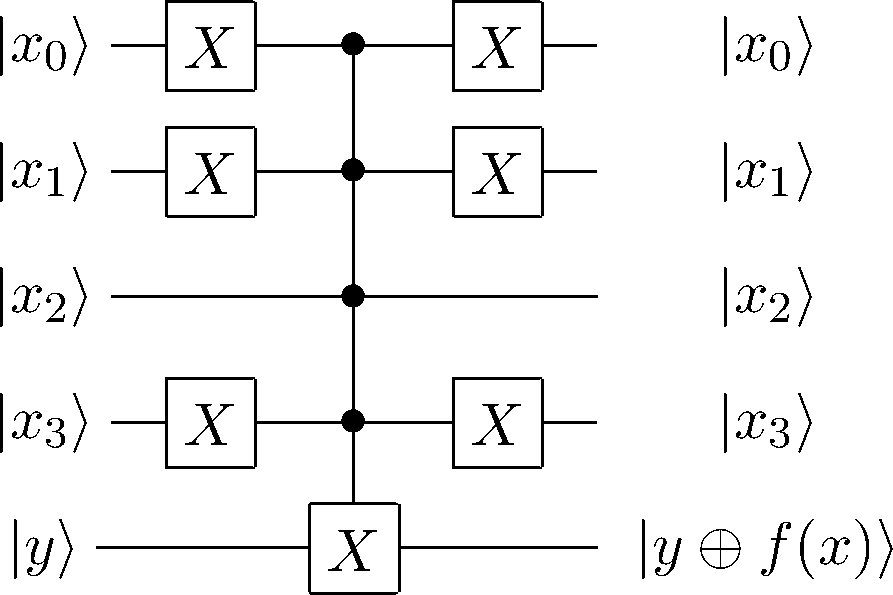
\includegraphics[width=0.25\textwidth]{oracle0010}
	\caption{A unitary function, setting the last qubit to 1 when 0010 is inputted, and 0 otherwise}
\end{figure}

This can be modified so that the overall state's sign is changed if $x = a$ by first setting the output qubit to $\ket{1}$ and applying the Hadamard gate to it before the application of $U_f$. So, the output qubit is in the state $H\ket{1} = \frac{1}{\sqrt{2}}(\ket{0} - \ket{1}) = \ket{-}$ before application, and after applying $U_f$ the overall state becomes
$$U_f(\ket{x} \oplus \ket{-}) = (-1)^{f(x)}\ket{x} \oplus \ket{-}$$
From this equation it is obvious that applying $U_f$ to the state is the same as doing nothing to the single output qubit, while applying a unitary transformation $V$ to the input register, where
\begin{equation}
	V\ket{x} = (-1)^{f(x)}\ket{x} = \begin{cases}
		\ket{x}, \quad x \neq a,\\
		-\ket{a}, \quad x = a.
	\end{cases}
\end{equation}

If we initially transform the n-qubit input register into a uniform superposition of all possible inputs, i.e.
$$\ket{\phi} = H^{\otimes n}\ket{0}_n = \frac{1}{2^{n/2}}\sum_{x=0}^{2^n-1}\ket{x}_n$$
Then, after applying $V$, the component of the state along $\ket{a}$ (i.e. the state we are looking for) will have a negative phase. The unitary $V$ can therefore be written as
$$V\ket{\Psi} = \ket{\Psi} - 2 \ket{a}\braket{a | \Psi} \qquad \therefore V = 1 - 2\ket{a}\bra{a}$$
\begin{figure}[H]
	\centering
	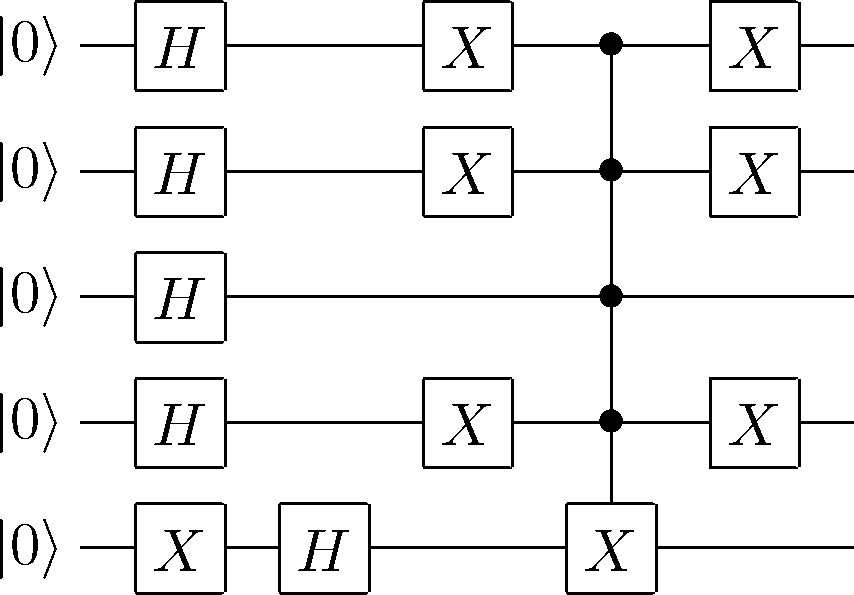
\includegraphics[width=0.25\textwidth]{oracle00102}
	\caption{Applying $V$ to an equal superposition of all possible inputs.}
\end{figure}

\paragraph{Implementation}
Before actually implementing the oracle used for Grover's algorithm in Haskell, it is useful to first define a few functions to work over lists of qubits - allowing easy expansion to custom oracles later on.
\begin{verbatim}
mkQbits :: Int -> Bool -> QIO [Qbit]}
mkQbits n b = mkQbits' n b []
  where
    mkQbits' 0 _ qs = return qs
    mkQbits' n b qs = do
      q <- mkQbit b
      mkQbits' (n-1) b (qs ++ [q])
\end{verbatim}

As you can see, \texttt{mkQbits} is a function which uses recursion to create a list of \texttt{n Qbit}s in the state given by \texttt{b}. This leads on to the creation of another function, \texttt{measQbits :: [Qbit] -> QIO [Bool]} which returns a list of boolean values representing the measurements of the inputted list of \texttt{Qbit}s. The only two remaining functions necessary pertain to applying unitary functions to lists of \texttt{Qbit}s. More specifically, we need a function which applies a single-qubit unitary operation to all qubits in a list, and another function which applies a single-qubit unitary operation to the last qubit in a list, conditional on the state of each other qubit in said list.
\begin{verbatim}
unitaryN :: (Qbit -> U) -> [Qbit] -> U
unitaryN _ []      = mempty
unitaryN uf (q:qs) = uf q <> unitaryN uf qs

condN :: (Qbit -> U) -> [Qbit] -> U
condN uf (q:[]) = uf q
condN uf (q:qs) = cond q (\x -> if x then (condN uf qs) else mempty)
\end{verbatim}

Now that these functions are created, initializing the qubits and applying the oracle is simple. First, we need to create $i$ qubits for each variable in the function and put them in the state $\ket +$, and then create $o$ qubits for each ``line'' in the function, each put in the state $\ket -$.

\begin{verbatim}
initialize :: Int -> Int -> QIO ([Qbit], [Qbit])
initialize i o = do
  qI <- mkQbits i False
  qO <- mkQbits o True
  applyU (unitaryN uhad (qI ++ qO))
  return (qI, qO)
\end{verbatim}

Now we need to create a function representing $V$, the oracle unitary. For now, this will be for the example above, searching for the state $\ket{110}$. 

\begin{verbatim}
oracle :: [Qbit] -> [Qbit] -> U
oracle qI qO =
  unot (qI!!2) <>
  condN unot (qI ++ [qO!!0]) <>
  unot (qI!!2)
\end{verbatim}

\subsubsection{Diffusion}
Grover's algorithm requires one more unitary $W$, which does not depend on the oracle function. This unitary transformation changes the sign of the component orthogonal to $\ket{\phi}$, i.e.
$$W = 2\ket{\phi}\bra{\phi} - 1$$
The unitary $-W$ works fine here, as the final state will only differ by an overall minus sign, if it differs at all. From $-W$, and the fact that the Hadamard gate is its own inverse, you can see that we need a gate which does nothing for all states apart from $\ket{00...00}$, which it multiplies by -1.
$$-W = 1 - 2\ket{\phi}\bra{\phi}, \qquad \ket{\phi} = H^{\otimes n}\ket{0}_n$$
$$\therefore -W = H^{\otimes n}(1 - 2\ket{00...00}\bra{00...00})H^{\otimes n}$$
\par
The Pauli-Z gate is the main gate to use here. This gate, with matrix 
$\begin{bmatrix}
	1 & 0 \\
	0 & -1
\end{bmatrix}$
, multiplies the state $\ket{11...11}$ by -1, and does nothing on all other states. From this, it is easy to see that if we applied a controlled Pauli-Z gate to the qubits, surrounded by $n$ Pauli-X gates, we get the unitary $-W$.
$$-W = H^{\otimes n} X^{\otimes n} (c^{n-1}Z) X^{\otimes n} H^{\otimes n}$$

\paragraph{Implementation} 
Implementing this is extremely simple using the functions created earlier, as shown below

\begin{verbatim}
diffuse :: [Qbit] -> U
diffuse qI =
  unitaryN uhad qI <>
  unitaryN unot qI <>
  condN (\q -> uphase q pi) qI <>
  unitaryN unot qI <>
  unitaryN uhad qI
\end{verbatim}

\subsubsection{Application \& Measurement}
All that is left now is to apply $WV$ repeatedly to the intital state $\ket{\phi}$ enough times for a solution state to be found. This is best described using simple geometry.\par

\begin{wrapfigure}{l}{0.55\textwidth}
\centering
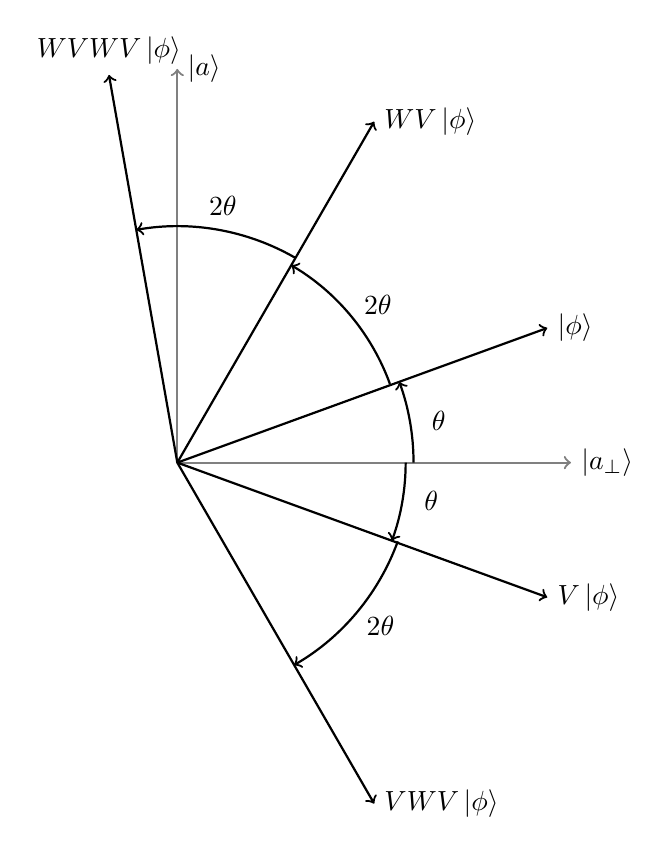
\begin{tikzpicture}
    \coordinate (origin) at (0,0);
    \draw[thick,gray,->] (origin) -- (5,0) node [black,right] {$\ket{a_\perp}$};
    \draw[thick,gray,->] (origin) -- (0,5) node [black,right] {$\ket{a}$};
    \draw[thick,black,->] (origin) -- (20:5) node [black,right] {$\ket{\phi}$};
    \draw[thick,black,->] (origin) -- (-20:5) node [black,right] {$V\ket{\phi}$};
    \draw[thick,black,->] (origin) -- (60:5) node [black,right] {$WV\ket{\phi}$};
    \draw[thick,black,->] (origin) -- (-60:5) node [black,right] {$VWV\ket{\phi}$};
    \draw[thick,black,->] (origin) -- (100:5) node [black,above] {$WVWV\ket{\phi}$};
    
    \draw[thick, black, ->] (3,0) arc (0:20:3) node [black,xshift=0.5cm,yshift=-0.5cm] {$\theta$};
    \draw[thick, black, ->] (2.9,0) arc (0:-20:2.9) node [black,xshift=0.5cm,yshift=0.5cm] {$\theta$};
    \draw[thick, black, ->] (2.7,1) arc (20:59.5:2.9) node [black,xshift=1.1cm,yshift=-0.5cm] {$2\theta$};
    \draw[thick, black, ->] (2.8,-1) arc (-20:-60:3) node [black,xshift=1.1cm,yshift=0.5cm] {$2\theta$};
    \draw[thick, black, ->] (1.5,2.6) arc (60:100:3) node [black,xshift=1.1cm,yshift=0.3cm] {$2\theta$};
\end{tikzpicture}
\end{wrapfigure}

The intial state $\ket{\phi}$ will contain one state $\ket{a}$ with amplitude $\frac{1}{2^{n/2}} = 1 / \sqrt{N}$, and so starts out at an angle $\theta$ from $\ket{a_\perp}$, where $\sin{\theta} = 1 / \sqrt{N}$.\par
The unitary $V$ negates the state $\ket{a}$ in $\ket{\phi}$, and so on the graph, it reflects $\ket{\phi}$ about the axis $\ket{a_\perp}$. Next, the unitary $W$ is applied which negates any state orthogonal to $\ket{\phi}$ (i.e. any negative state in $\ket{\phi}$, notably the state $\ket{a}$). Graphically, this means the unitary $W$ reflects about $\ket{\phi}$, and so when applied to $V\ket{\phi}$, it results in a state at an angle of $3\theta$ above $\ket{a_\perp}$. Therefore, each iteration (application of the unitary $V$ followed by $W$) rotates the qubits' state by $2\theta$ anti-clockwise, giving us a simple method to find out the amount of iterations, $i$, required. Note: when N is large, $\sin{\theta} \approx \theta$.
$$\theta + 2i\theta \approx \pi / 2  \qquad \sin{\theta} = 1 / \sqrt{N} \qquad \therefore \theta \approx 1 / \sqrt{N}$$ 
$$\therefore i \approx \frac{\pi - 2\theta}{4\theta} \approx \frac{\pi}{4} \sqrt{N}$$
\par
The amplitude of the state $\ket{a}$ over the qubits is given by the sine of the angle between the qubits and $\ket{a_\perp}$, and so the probability of measuring the solution from the qubits is equal to the square of this.

\paragraph{Example}
Say we want to search for $\ket{110}$ across a space of 8 (i.e. 3 qubits). The iterations required will therefore be $\approx \frac{\pi}{4} \sqrt{8} \approx 2$. The oracle function will perform a controlled-X gate on its output qubit if its inputs are in the state $\ket{110}$. Then, we need to diffuse the qubits using the unitary $W$ described above. After initializing the qubits, we must apply $V$, then $W$, and repeat this again to get a solution. 
\begin{figure}[H]
    \centering
    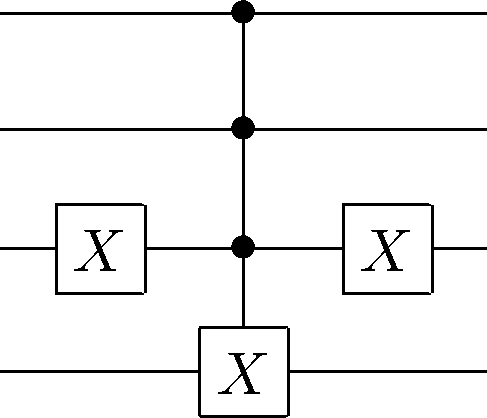
\includegraphics[width=0.25\textwidth]{grovers110V}
    \hspace{1cm}
    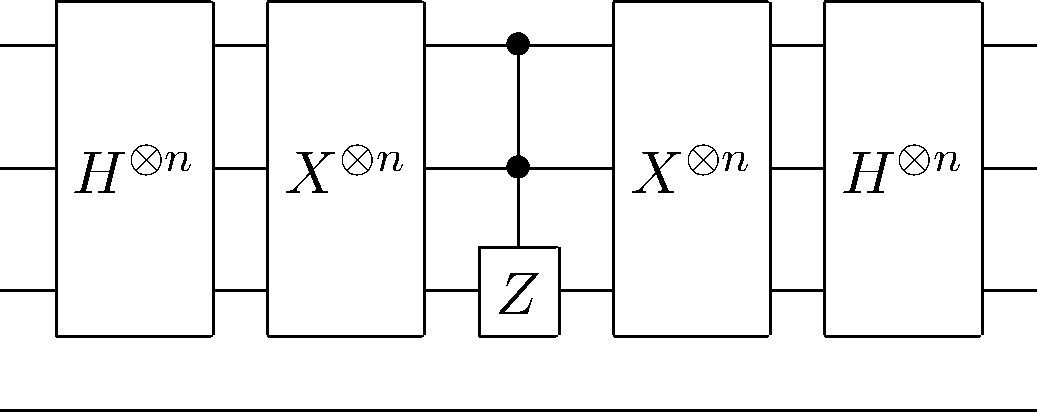
\includegraphics[width=0.5\textwidth]{grovers110W}
    \caption{The 2 unitaries $V$ (left) and $W$ (right) used to search for $\ket{110}$.}
\end{figure}
\begin{figure}[H]
    \centering
    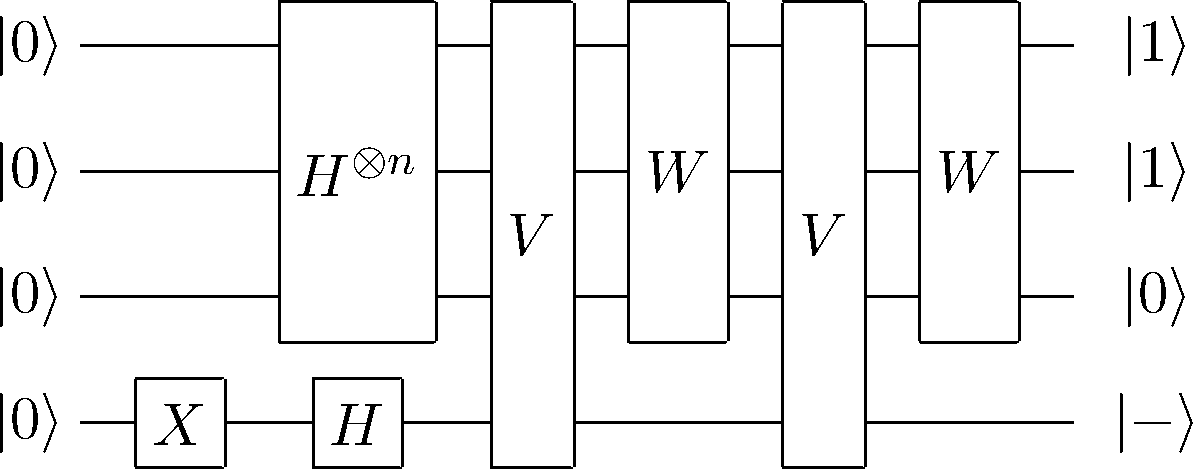
\includegraphics[width=0.5\textwidth]{grovers110}
    \caption{The circuit used to perform Grover's algorithm over 3 input qubits, with solution $\ket{110}$.}
\end{figure}

\paragraph{Implementation}
All that remains in the implementation is to combine the functions described above and apply them the correct amount of times (i.e. twice when searching for the state $\ket{110}$).

\begin{verbatim}
grover :: QIO [Bool]
grover = do
  (qI, qO) <- initialize 3 1
  let groverStep = oracle qI qO <> diffuse qI
  applyU (groverStep)
  applyU (groverStep)
  measQbits qI  
\end{verbatim}

\paragraph{Testing}
Testing this is relatively simple: simply \texttt{run} the \texttt{grover} function, check the result and then \texttt{sim} the function, checking the probability of expected results.\par
\begin{verbbox}
run grover -> [True, True, False]
sim grover -> [..., ([True, True, False], 0.9453125), ...]
\end{verbbox}

\begin{figure}[H]
    \centering
    \theverbbox \\
    with all other states having probability $7.812...e^{-3}$
\end{figure}

\subsubsection{Expansion to multiple solutions}
The algorithm above can also search for multiple solutions, the only thing that changes is the amount of iterations necessary. If there are $s$ solutions, then the amount of iterations required becomes $i \approx \frac{\pi}{4} \sqrt{\frac{N}{s}}$.\par

\subsubsection{Implementing a Custom Oracle}
In the example above, the oracle is searching for \texttt{True, True, False}, i.e. $x1 \land x2 \land \neg x3$. So, if the program takes in a function as a boolean predicate, it can create a unitary function representing the oracle using a list of the input variables in the predicate, and applying 2 NOT gates to negated variables.\par
The oracle can also search for multiple lines of predicates separated by OR operations; simply have a different output qubit for each line, so that solutions to every line will be negated, allowing easy usage for multiple solutions. For example, if the user wants to apply the algorithm over a function $f$, where
$$f(x_n) = (x1 \land x2 \land x3) \lor (\neg x1 \land x2 \land \neg x3)$$
then they can input\par
\begin{verbbox}
1 2 3
-1 2 -3
\end{verbbox}
\begin{figure}[H]
    \centering
    \theverbbox
\end{figure}

So the oracle function needs to be changed to take in a list of a list of \texttt{Int}s, i.e. \texttt{[[Int]]}, where each inner list represents a line of the function. From this, it will recursively apply the NOT gates over qubits referenced by negative integers, and apply controlled-X gates over the qubits referenced in each line to the output qubits, where each inner list is applied to its own unique output qubit.\par
\begin{verbatim}
oracle :: Int -> [[Int]] -> [Qbit] -> [Qbit] -> U
oracle _ [] _ _ = mempty
oracle c (p:ps) qI qO =
  unitaryN unot (unots p qI) <>
  condN unot (conds p qI ++ [q0!!c]) <>
  unitaryN unot (unots p qI) <>
  oracle (c+1) ps qI q0
  where
    unots p qI = map (\x -> qI!!((abs x)-1)) $ filter (< 0) p
    conds p qI = map (\x -> qI!!((abs x)-1)) p
\end{verbatim}

The program also needs to know how many solutions there are in order to iterate the application of $V$ and $W$ the correct amount of times, roughly equal to $\frac{\pi}{4}\sqrt{\frac{N}{s}}$. The application can then be done using the \texttt{foldr} function, folding with the \texttt{mappend} operator \texttt{<>}, starting from \texttt{mempty}.\par
The entry point to the algorithm will be using the \texttt{main} function in the code. This function, of type \texttt{IO ()}, will take in a custom function inputted in the form described above, and then run the algorithm over it. This can also be timed effectively using the \texttt{TimeIt} package \cite{timeit}.

\subsubsection{Testing}
In order to test this, the program needs to be changed slightly to \texttt{sim} the algorithm, and print out the probabilities. The above predicate $x1 \land x2 \land \neg x3$, inputted as \texttt{1 2 -3} returns the expected result:

\begin{verbbox}
[...,([True, True, False]), 0.9453125),...]
\end{verbbox}

\begin{figure}[H]
    \centering
    \theverbbox
    \\ with all other states having probability $7.812...e^{-3}$
\end{figure}

A more complicated predicate shown below also returns the correct result, indicating the implementation works correctly. 
$$(x1 \land \neg x2 \land x3 \land x4) \lor (x2 \land \neg x3 \land x4) \lor (x1 \land x2 \land x3)$$
\begin{center}
Solutions: $0101, 1011, 1101, 1110, 1111$\\
Output: \\\texttt{[([True, True, True, True], 0.1914...),\\ ([True, True, True, False], 0.1914...),\\ ([True, True, False, True], 0.1914...),\\...,\\ ([True, False, True, True], 0.1914...),\\...,\\ ([False, True, False, True], 0.1914...), \\...]} with all other states having probability $3.906...e^{-3}$
\end{center}

\subsubsection{An Improvement}
This algorithm can be altered to actually not use any ancilla qubits in QIO  (due to the way QIO executes multi-qubit gates) and use less gates, improving run time. The current implementation uses ancilla qubits to negate solution states in the input qubits. However, this can simply be done using a controlled Pauli-Z gate over the inputs, when the input qubits are initially in the state $\ket{-}$. After this, the diffusion is also simplified to become an inversion about the mean \cite{groverblog}; decrease the amplitude of non-solutional states about the mean amplitude while increasing the amplitude of solutional states. This can be achieved by $n-1$ Hadamard gates surrounding a $C^n$-NOT gate.\par

\begin{figure}[H]
    \centering
    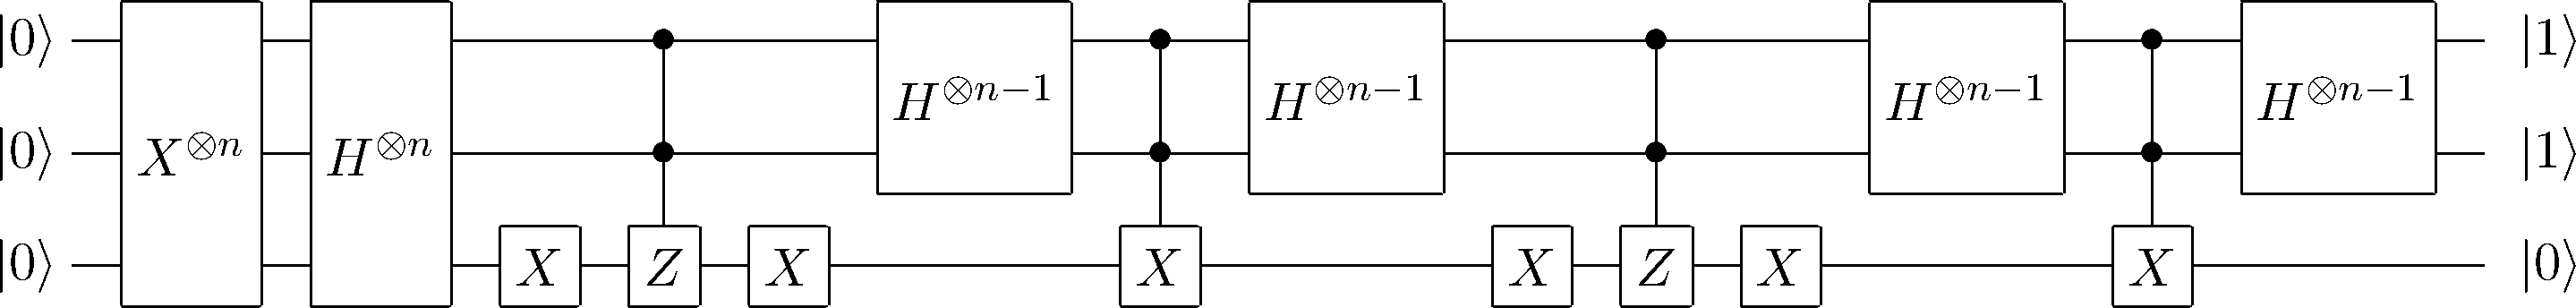
\includegraphics[width=\textwidth]{groverImp}
    \caption{Improved circuit for Grover's algorithm, searching for the state $\ket{110}$}
\end{figure}

In order to change the code to implement this, the \texttt{initialize}, \texttt{oracle} and \texttt{diffuse} functions need to be altered.

\subsubsection{Testing Solutions}
The current algorithm works well when solving a function with a known amount of solutions, and returns correct solutions with a high probability as shown. However, the implementation can be changed to measure whether or not the input qubits contain a solution at the end, This will enable the program to return definite, distinct solutions and find solutions to functions with an unknown amount of solutions.\par
By simply using ancilla qubits to test the state of input qubits with $C^n$-NOT gates, a final ancilla qubit will be in the state $\ket{1}$ if the input qubit's contain a solution.

\begin{figure}[H]
    \centering
    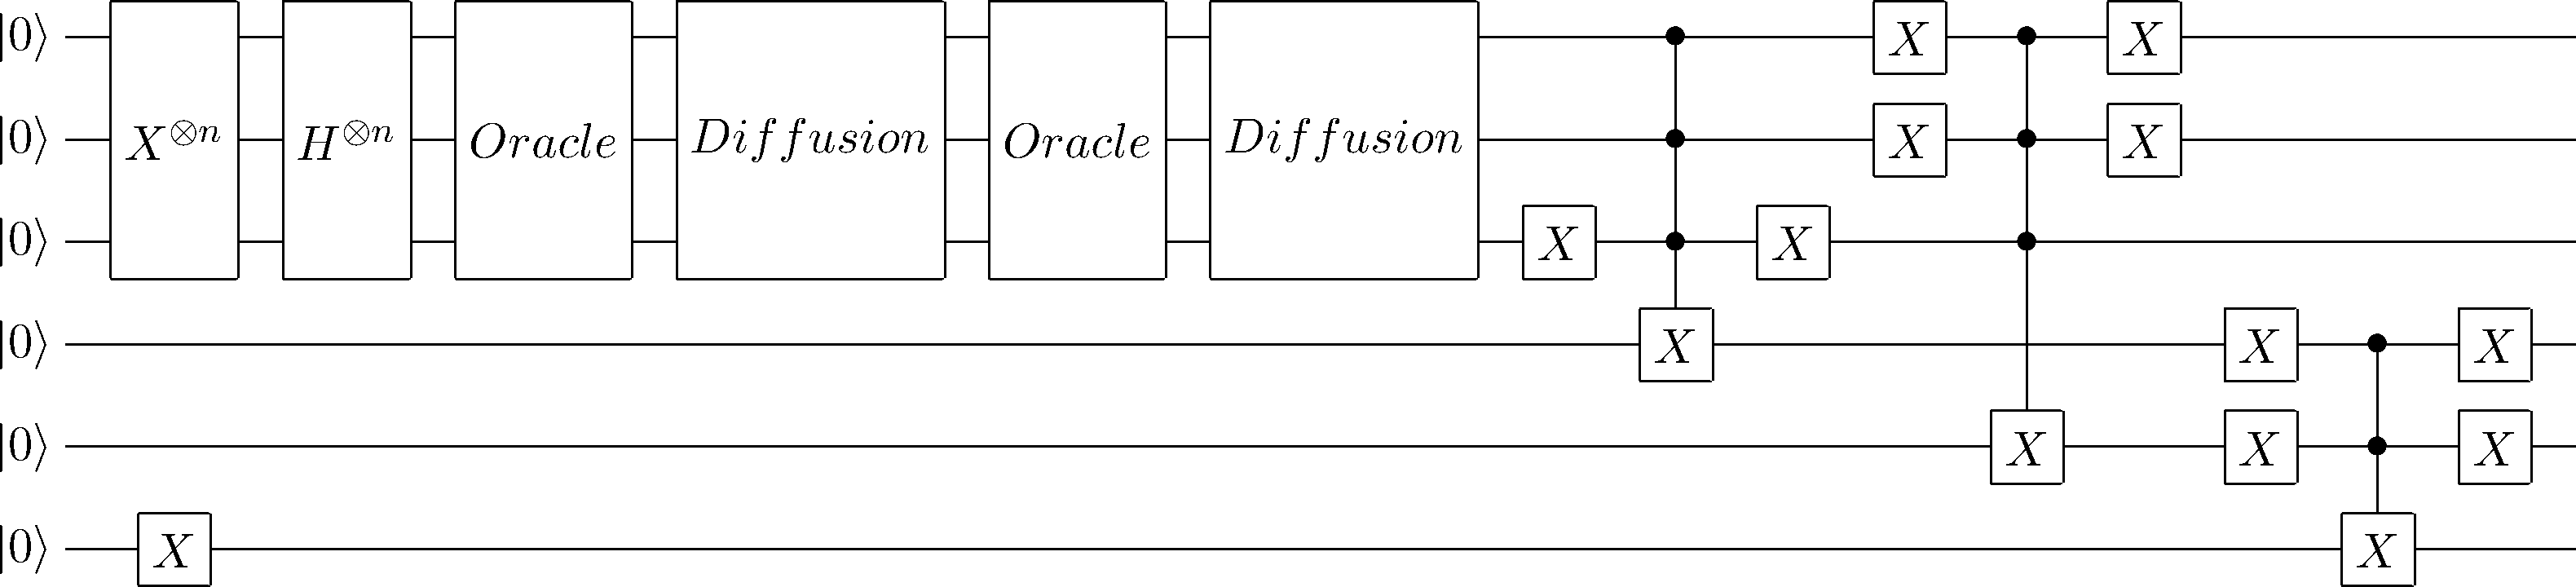
\includegraphics[width=\textwidth]{groverFinal}
    \caption{Improved circuit for Grover's algorithm, searching for the state $\ket{110}$ and $\ket{001}$, while also checking $n$ qubits for the solution.}
\end{figure}
The results of each line of the function (i.e. $x0 \land x1 \land \neg x2$ and $\neg x0 \land \neg x1 \land x2$) are saved into two separate qubits. Following this, a third ancilla qubit is set to $\ket{0}$ if both the two ancilla qubits are in the state $\ket{0}$, which would only occur when the input qubits do not contain a solution.

\paragraph{Implementation}
In order to implement this, the \texttt{initialize} function will need create the necessary ancilla qubits, all of which will be in the state $\ket 0$ except for the last, which will be in the state $\ket 1$. A new function needs to be created to apply the necessary $C^n$-NOT gates over the input qubits on distinct ancilla qubits, which will be applied after the algorithm has been executed. Finally, the program will measure the last ancilla qubit in the list, and return this with the measurements of the input qubits. The ancilla measurement can then be checked to determine if a solution was found, allowing easy looping to get multiple, unique and definite solutions. \par
This will also enable the algorithm to be used for functions with an unknown amount of solutions, as this requires multiple executions of the algorithm with differing amounts of iterations until a solution is found. In this case, the amount of iterations starts as $\frac{\pi}{4}\sqrt{N}$. If this does not result in a solution, the algorithm is executed again with $\frac{\pi}{4}\sqrt{\frac{N}{2}}$ iterations, and then $\frac{\pi}{4}\sqrt{\frac{N}{4}}$ iterations, and so on until a solution is found. The total amount of iterations required is still $O(\sqrt N)$ as shown below.
$$\frac{\pi}{4}\sqrt N \left(1 + \frac{1}{\sqrt 2} + \frac{1}{2} + \frac{1}{2\sqrt 2} + ...\right) = \frac{\pi}{4}\sqrt N \sum_{i=0}^{\infty}\frac{1}{2^i} = \frac{\pi}{4}\sqrt N (2 + \sqrt 2)$$

\subsubsection{Probability}
We can also print out the probability of finding the solution by running the \texttt{sim} function over a function which only measures the last ancilla qubit (which will only be measured to be True if the input qubits contain a solution).

\begin{verbatim}
probability :: Int -> Int -> [[Int]] -> IO ()
probability n i ps = putStrLn $ show $ sim $ probOfSolution
  where
    probOfSolution = do
      (qI, qA) <- initialize n ((length ps)+1)
      let groverStep = oracle ps qI <> diffuse qI
      applyU (foldr (<>) mempty (replicate i groverStep))
      applyU (testForSolution 0 ps qI qA)
      measQbit $ last qA
\end{verbatim}

\subsection{Shor's Algorithm}
As mentioned in section 4.1, there is already an implementation of Shor's algorithm in QIO, in the file \texttt{Shor.hs}. Therefore, this section will be dedicated to explaining the current implementation, and describing any potential improvements.\par
In section 4.2.2, it was stated that Shor's algorithm is for integer factorization. This is not exactly correct, as the algorithm actually finds the period of a function, which can then be expanded to factorize integers. Let $f$ be a function, periodic on addition, over integers, i.e.\par
$$f(x) \equiv f(y) \iff x = y + cr, \qquad c \in \mathbb{Z} $$
Classical algorithms for finding the period of such a function take a time which grows faster than any power of the number of bits of $r$. However, Shor's algorithm does this in a time which scales slightly faster than $n^3$ \cite{qscbook}\textsuperscript{Page 63}.\par
Put simply, the algorithm applies the function $f$ over two qubit registers. Measuring the second register, i.e. the register containing the results of $f(x)$, collapses the first into a superposition over all the values which give that measured value. Each of these values in the register will be separated by integer multiples of the period $r$. Finally, we apply an algorithm known as the quantum Fourier transformation, which extracts the value of the period $r$ from the register. We can then measure this register to obtain a value for the period. Similar to Grover's algorithm, it can be broken down into distinct parts:\par
\begin{enumerate}
    \item \textbf{Function Application} - Creating a unitary representation for the function $f$, and applying it to the two qubit registers.
    \item \textbf{QFT} - Applying the quantum Fourier transformation to the first register after measuring the second.
    \item \textbf{Period finding} - Measuring the second register and calculating a value for the period $r$.
\end{enumerate}
In order expand this to factorize an integer $N = pq$, where $p$ and $q$ are 2 prime numbers, the function to apply is
$$f(x) = b^x \Mod N, \text{ where $b$ is coprime to $N$}$$
The required amount of qubits in each register is equal to the number of bits in $N$, namely $n_0$. However, to efficiently find the period $r$, the input register needs to actually have twice this amount, ensuring the range of values for $x$ on which $f(x)$ is calculated has at least $N$ full periods of $f$\cite{qscbook}\textsuperscript{Page 69}. After applying Shor's algorithm with the above function, the period $r$ needs to have certain properties
\begin{enumerate}
    \item $r$ needs to be even so we can calculate
    $$x = b^{\frac{r}{2}}\Mod N$$
    \item $x-1 \neq 0 \Mod N$ as $r$ must be the smallest integer for which $b^r = 1 \Mod N$
\end{enumerate}
From this,
$$ x^2 = (b^{\frac{r}{2}})^2 \Mod N = b^r \Mod N = 1 \Mod N$$
$$\therefore (x-1)(x+1) = x^2 - 1 = 0 \Mod N$$
So now, $(x-1)$ and $(x+1)$ aren't divisible by $N$, but $(x-1)(x+1)$ is. As $N$ is the product of 2 primes, $p$ and $q$, it follows that $(x-1)$ is divisble by $p$, and $(x+1)$ is divisble by $q$. Therefore, $p = gcd(x-1, N)$ and $q = gcd(x+1, N)$.

\subsubsection{Function Application}
\paragraph{Calculating U\textsubscript{f}} So, we need a unitary $U_f$ which calculates $f(x) = b^x \Mod N$, i.e.
$$U_f \ket{x} \otimes \ket{y} = \ket x \otimes \ket{y \oplus f(x)}$$
Doing this is actually fairly simple: square $b \Mod N$, then square the result $\Mod N$, then square that etc. calculating the number of powers $b^{2^j} \Mod N$ where $j < n$. So, if initially $x$ is in the input register, $1$ (i.e. $00..01$) is in the output register, and $b$ is in an additional work register, then the process is simple\cite{qscbook}\textsuperscript{Page 84}:
\begin{enumerate}
    \item Multiply the output register by the work register using modular multiplication if $x_0 = 1$,
    \item Replace the contents of the work register by its modulo-N square,
    \item Repeat step 1, now conditional on $x_1 = 1$,
    \item Repeat step 2,
    \item Repeat step 1, now conditional on $x_2 = 1$, etc.
\end{enumerate}
At the end of this, $x$ will still be in the input register, and $b^x \Mod N$ will be in the output register.

The current implementation of this, found in \texttt{QArith.hs}, uses a combination of modular addition operations to form modular multiplication operations, which in turn are combined together to form modular exponentiation operations, calculating $f(x)$. This is explained in the G53/G54NSC ``Shor's Algorithm continued...'' lecture \cite{nsc}. 

\paragraph{Applying U\textsubscript{f}}
Applying the above unitary to the state $\ket \phi _n \otimes \ket 0 _{n_0}$, where 
$$\ket \phi _n =H^{\otimes n} \ket 0 = \frac{1}{2^{n/2}} \sum_{x=0}^{2^n -1} \ket x$$
results in the state
$$\frac{1}{2^{n/2}} \sum_{x=0}^{2^n -1} \ket x _n \ket{f(x)}_{n_0}$$
If we then measure the output register to be $f_0$, the state of the input register will collapse to containing all of the values which give the same value for $f(x)$, i.e.
$$\ket \Psi _n = \frac{1}{\sqrt m} \sum _{k=0}^{m-1} \ket{x_0 + kr}_n, \qquad  0 \leq x_0 < r, \qquad f(x_0) = f_0 $$ where $m$ is the smallest integer where $mr + x_0 \geq 2^n$, and so
$$m = \left[ \frac{2^n}{r} \right] \text{ or } m = \left[ \frac{2^n}{r} \right] + 1 \text{, where $\left[ \frac{2^n}{r} \right]$ is the largest integer less than or equal to $\frac{2^n}{r}$} $$
Measuring this register right now would give us a value for $x_0 + kr$, where $x_0$ is unknown and random, and so we cannot calculate the value of $r$ yet. We first need to remove the $x_0$ from the state using the quantum Fourier transform.

\subsubsection{The Quantum Fourier Transform}
Periodic functions can be decomposed into the sum of simple sine and cosine functions, and this decomposition is calculated by the Fourier transform. The discrete Fourier transform from the vector $x_0, x_1, ..., x_{2^n -1}$ to the vector $y_0, y_1, ..., y_{2^n -1}$ is defined by
$$y_a = \frac{1}{\sqrt{2^n}} \sum _{b=0}^{2^n -1} e^{2\pi iab/2^n} x_b $$
\par
This can be used to our advantage. In order to remove the $x_0$ value from the state described above, the quantum Fourier transform is used to turn it into a harmless overall phase factor, allowing us to get the value for the period $r$. The equation for the quantum Fourier transform unitary $U_{FT}$ is shown below
$$U_{FT} \ket x _n = \frac{1}{2^{n/2}}\sum _{y=0}^{2^n -1} e^{2\pi ixy/2^n} \ket y _n$$
When applied to a superposition of states $\ket x$ with complex amplitudes $\gamma (x)$, $U_{FT}$ produces another superposition with amplitudes related to $\gamma (x)$ by the appropriate discrete Fourier transform
$$U_{FT} \left( \sum _{x=0}^{2^n -1} \gamma (x) \ket x \right) = \sum _{x=0}^{2^n -1} \tilde{\gamma} (x), \ket x \qquad \text{where } \tilde{\gamma} (x) = \frac{1}{2^{n/2}} \sum _{y=0}^{2^n -1} e^{2\pi ixy/2^n} \gamma (y)$$
Now, in order to construct the quantum Fourier transform circuit, it is best to define a unitary $U_Z$, which can be seen as a generalization of the Pauli-Z gate to $n$ qubits, where
$$U_Z \ket y _n = e^{2\pi iy/2^n} \ket y _n$$ 
From this, it is clear that
$$U_Z ^x H^{\otimes n} \ket 0 _n = U_Z ^x \left( \frac{1}{2^{n/2}} \sum _{y=0}^{2^n -1} \ket y _n \right) = \frac{1}{2^{n/2}} \sum _{y=0}^{2^n -1} e^{2\pi ixy/2^n} \ket y _n = U_{FT} \ket x _n$$
In order to make the construction even easier, we can look at a specific case, say $n = 4$, and then generalize for any value of $n$. So, $n = 4$ means
$$U_{FT} \ket{x_3}\ket{x_2}\ket{x_1}\ket{x_0} = U_Z^x H_3 H_2 H_1 H_0 \ket 0 \ket 0 \ket 0 \ket 0$$
If $\ket y _4 = \ket{y_3} \ket{y_2} \ket{y_1} \ket{y_0}$, then $y = 8y_3 + 4y_2 + 2y_1 + y_0$. Now we can construct $U_Z$ using its definition above.
$$U_Z y = e^{\pi i/8} (8y_3 + 4y_2 + 2y_1 + y_0)$$
$$\therefore U_Z = \text{exp} \left( \frac{\pi i}{8} (8\text{n}_3 + 4\text{n}_2 + 2\text{n}_1 + \text{n}_0)\right)$$
$$\therefore U_Z^x = \text{exp} \left( \frac{\pi i}{8} (8x_3 + 4x_2 + 2x_1 + x_0)(8\text{n}_3 + 4\text{n}_2 + 2\text{n}_1 + \text{n}_0)\right)$$
We can simplify this, combining the coefficients for each n.
\begin{align*}
U_Z^x = \text{exp} (\pi i (&\text{n}_3 (8x_3 + 4x_2 + 2x_1 + x_0) +\\
&\frac{1}{2}\text{n}_2 (8x_3 + 4x_2 + 2x_1 + x_0) + \\
&\frac{1}{4}\text{n}_1 (8x_3 + 4x_2 + 2x_1 + x_0) + \\
&\frac{1}{8}\text{n}_0 (8x_3 + 4x_2 + 2x_1 + x_0))
\end{align*}
Now, the unitary operation exp$(2\pi i$n$)$ is the same as a two Pauli-Z gates, and so is simply an identity operator. This means any exp$(2^p\pi i$n$)$ can be removed, allowing us to further simplify $U_Z^x$
$$U_Z^x = \text{exp} \left(\pi i (x_0\text{n}_3 + (x_1 + \frac{1}{2}x_0)\text{n}_2 + (x_2 + \frac{1}{2}x_1 + \frac{1}{4}x_0)\text{n}_1 + (x_3 + \frac{1}{2}x_2 + \frac{1}{4}x_1 + \frac{1}{8}x_0)\text{n}_0\right)$$
Following this, we can simply the equation for $U_Z ^x H^{\otimes x} \ket 0 _n$. The operators exp$(\pi i x$n$)$ and $H\ket 0$ obey the relation $\text{exp}(\pi i x \text{n}) H\ket 0 = H\ket x$ over single qubits.
For now, lets ignore the terms with fractional coefficients.
\begin{align*}
\text{exp}& (\pi i (x_0\text{n}_3 + x_1\text{n}_2 + x_2\text{n}_1 + x_3 \text{n}_0)H_3 H_2 H_1 H_0 \ket 0 \ket 0 \ket 0 \ket 0 \\
= &\text{  }[\text{exp}(\pi i x_0 \text{n}_3)H_3\ket 0 ]\text{  }[\text{exp}(\pi i x_1 \text{n}_2)H_2\ket 0 ]\text{  }[\text{exp}(\pi i x_2 \text{n}_1)H_1\ket 0 ]\text{  }[\text{exp}(\pi i x_3 \text{n}_0)H_0\ket 0 ] \\
= &\text{  }[H_3 \ket{x_0}]\text{  }[ H_2 \ket{x_1}]\text{  }[ H_1 \ket{x_2}]\text{  }[ H_0 \ket{x_3}]\\
= & \text{  }H_3 H_2 H_1 H_0 \ket{x_0} \ket{x_1} \ket{x_2} \ket{x_3}
\end{align*}
When we add in and group the remaining terms we are left with the following
\begin{align*}
U_{FT} \ket{x_3} \ket{x_2} \ket{x_1} \ket{x_0} = & H_3 \text{ exp}\left[\pi i \text{n}_2 \frac{1}{2} x_0 \right]H_2 \text{ exp}\left[\pi i \text{n}_1 \left(\frac{1}{2} x_1 + \frac{1}{4}x_0 \right) \right]H_1 \\
& \times \text{ exp}\left[\pi i \text{n}_0 \left(\frac{1}{2} x_2 + \frac{1}{4} x_1 + \frac{1}{8} x_0\right) \right]H_0\\
& \times \ket{x_0} \ket{x_1} \ket{x_2} \ket{x_3}
\end{align*}
The state $\ket{x_0} \ket{x_1} \ket{x_2} \ket{x_3}$ is an eigenstate of the number operators n\textsubscript{3}, n\textsubscript{2}, n\textsubscript{1}, n\textsubscript{0} with eigenvalues $x_0, x_1, x_2, x_3$, allowing us to simplify further.
\begin{align*}
U_{FT} \ket{x_3} \ket{x_2} \ket{x_1} \ket{x_0} = & H_3 \text{ exp}\left[\pi i \frac{1}{2} \text{n}_2 \text{n}_3 \right]H_2 \text{ exp}\left[\pi i \text{n}_1 \left(\frac{1}{2} \text{n}_2 + \frac{1}{4}\text{n}_3 \right) \right]H_1 \\
& \times \text{ exp}\left[\pi i \text{n}_0 \left(\frac{1}{2} \text{n}_1 + \frac{1}{4} \text{n}_2 + \frac{1}{8} \text{n}_3\right) \right]H_0\\
& \times \ket{x_0} \ket{x_1} \ket{x_2} \ket{x_3}
\end{align*}
After defining a new unitary operator for the 2-qubit operators, this becomes a lot clearer.
$$V_{ij} = \text{exp}(\pi i \text{n}_i \text{n}_j / 2^{|i - j|})$$
\begin{align*}
\therefore U_{FT}& \ket{x_3} \ket{x_2} \ket{x_1} \ket{x_0} \\
= & H_3 (V_{32}H_2)(V_{31}V_{21}H_1)(V_{30}V_{20}V_{10}H_0)\ket{x_0} \ket{x_1} \ket{x_2} \ket{x_3}
\end{align*}
It is obvious now that $V_{ij}$ simply rotates qubit $x_j$ by $e^{\pi i / 2^{|i-j|}}$ when the qubit $x_i$ is in the state $\ket 1$, allowing us to define a simple rotation operator.
$$R_k =
\begin{bmatrix}
    1 & 0\\
    0 & e^{\pi i / 2^k}
\end{bmatrix}
\text{, where } k = |i - j|
$$
All that is left is to define a unitary $S$, where $S\ket{x_3} \ket{x_2} \ket{x_1} \ket{x_0} = \ket{x_0} \ket{x_1} \ket{x_2} \ket{x_3}$ (made out of multiple SWAP operations), and we have a definition for $U_{FT}$ using 1 and 2 qubit gates.
$$U_{FT} = H_3 (R_{1}H_2)(R_{2}R_{1}H_1)(R_{3}R_{2}R_{1}H_0)S$$

\begin{figure}[H]
    \centering
    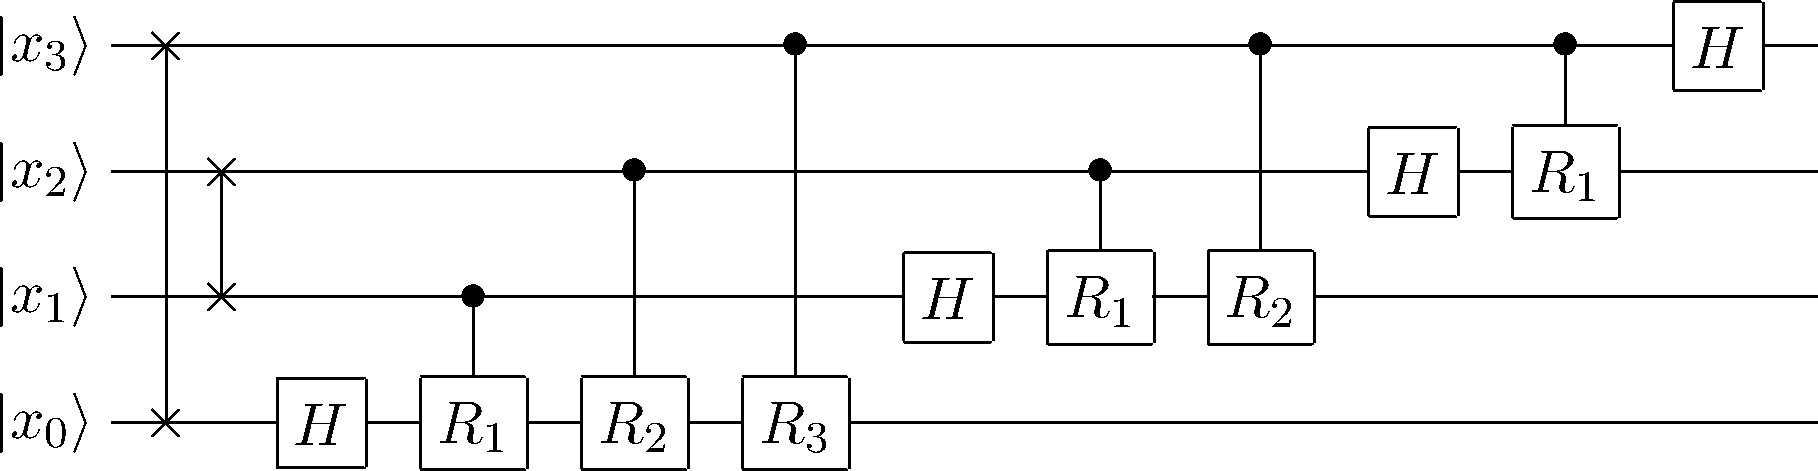
\includegraphics[width=0.8\textwidth]{qft}
    \caption{The circuit diagram for the quantum Fourier transform operation over 4 qubits}
\end{figure}

\paragraph{Implementation}
The implementation of the quantum Fourier transform in QIO is actually slightly different. By reversing the order of the controlled rotations, and the overall order of the gates, we can remove the need for SWAP operations at the start.
\begin{figure}[H]
    \centering
    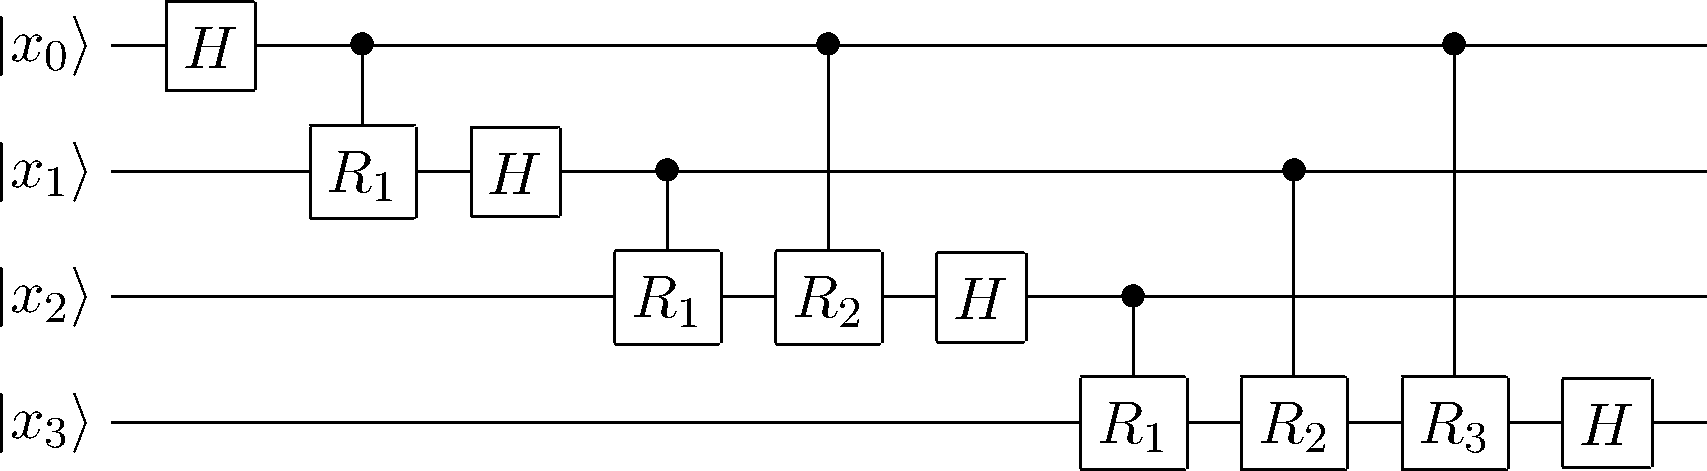
\includegraphics[width=0.8\textwidth]{qft2}
    \caption{The circuit diagram for an alternate quantum Fourier transform operation over 4 qubits}
\end{figure}

So, given a list of \texttt{Qbit}s, we need to apply a Hadamard gate, and then multiple rotation gates for each remaining \texttt{Qbit} in the list, where each gate is conditional on a distinct \texttt{Qbit}. I.e. given a list of 4 \texttt{Qbit}s, the unitary to construct is shown below, where \texttt{R k xn} is a $R_k$ gate on qubit $x_n$.
\begin{verbatim}
uhad x0 <> 
cond x0 (\x -> if x then R 1 x1 else mempty) <> uhad x1 <>
cond x1 (\x -> if x then R 1 x2) <> cond x0 (\x -> if x then R 2 x2) <> uhad x2 <>
cond x2 (\x -> if x then R 1 x3) <> cond x1 (\x -> if x then R 2 x3) <> 
cond x0 (\x -> if x then R 3 x3) <> uhad x3
\end{verbatim}

In order to create such a unitary operation, the implementation uses a recursive function which takes in 

\paragraph{Finding the period}
So, after applying the unitary $U_f$ to the state $\ket \phi _n \otimes \ket 0 _{n_0}$ we are left with the state
$$\frac{1}{2^{n/2}} \sum_{x=0}^{2^n -1} \ket x _n \ket{f(x)}_{n_0}$$
After measuring the output register, the input register collapses to the state
$$\ket \Psi _n = \frac{1}{\sqrt m} \sum _{k=0}^{m-1} \ket{x_0 + kr}_n, \qquad  0 \leq x_0 < r, \qquad f(x_0) = f_0 $$
To extract the period $r$, we can apply the quantum Fourier transformation as shown below.
\begin{align*}
    U_{FT}\ket \Psi &= \frac{1}{2^{n/2}}\sum_{y=0}^{2^n-1}\frac{1}{\sqrt m}\sum_{k=0}^{m-1}e^{2\pi i(x_0 + kr)y/2^n} \ket y \\
    & = \sum_{y=0}^{2^n-1}e^{2\pi i x_0y/2^n} \frac{1}{\sqrt{2^nm}}\left(\sum_{k=0}^{m-1}e^{2\pi i kry/2^n}\right) \ket y
\end{align*}
The probability of getting the result $y$ is therefore given by
$$\frac{1}{2^nm}\left| \sum_{k=0}^{m-1}e^{2\pi i kry/2^n}\right|^2$$
which is highest when $y$ is close to integral multiples of $2^n/r$. So, the period is given by the equation $r = 2^n / y$.

\paragraph{Factorizing N}
Now that we have a value for $r$, we need to check that it is even, and then calculate $x = b^{r/2} \Mod N$. After this, we need to check that $(x-1)$ is not divisible by $N$. If both these cases are true, we can factorize $N$, and if not we must find a new value for $r$ using a different value for $b$ for the application of $U_f$. \par
All that is left to do is find the greatest common divisor of $N$ and $x-1$, and $N$ and $x+1$, which will be the values of $p$ and $q$ in the equation $N = pq$.

\subsubsection{An alternative}
The quantum Fourier transformation has another use; it's inverse can be used in a procedure known as phase estimation. If we have a superposition of states
$$\frac{1}{2^{t/2}}\sum_{j=0}^{2^t-1}e^{2\pi i \varphi j} \ket j _n \ket u _m$$
we can apply the inverse quantum Fourier transform to get the state
$$\ket {\hat{\varphi}}_n \ket u _m \text{ where  $\hat{\varphi}$ is an approximation of $ \varphi $ up to $n$ bits.}$$\par
We can use phase estimation to execute Shor's algorithm with a higher accuracy. So, to recap, after applying $U_f$, we are left with the state
$$\frac{1}{2^{n/2}} \sum_{x=0}^{2^n -1} \ket x \ket{b^x \Mod N}$$
This state is approximately equal to 
$$\frac{1}{\sqrt{r2^n}}\sum_{s=0}^{r-1} \sum_{x=0}^{2^n-1} e^{2\pi i x \frac{s}{r}} \ket x \ket{u_s} \text{ where } \ket{u_s} = \frac{1}{\sqrt r} \sum_{k=0}^{r-1} e^{\frac{-2\pi isk}{r}} \ket{b^k \Mod N}$$
Applying the inverse quantum Fourier transform to this state gives
$$\frac{1}{\sqrt r}\sum_{s=0}^{r-1} \ket{( \frac{\hat s}{r} )} \ket{u_s}$$
and so measuring the first register will give us an integer result for $\varphi = \left( \frac{\hat s}{r} \right) $ up to $n$ bits. We can then use the continued fractions algorithm for $\frac{\varphi}{2^n}$ to calculate $r$.




Say we have a periodic function of $x$ with period $r$, where $N$ is the product of 2 primes, $p$ and $q$.
$$b^r = 1 \Mod N, \qquad r \in \mathbb{Z}, \qquad N = pq$$
$$\therefore f(x) = b^x \Mod N \implies f(x+s) = f(x) \Leftrightarrow s = cr, \qquad c \in \mathbb{Z} $$
In order to find a value for $b$, we all the numbers coprime with $N$, done simply using Euclid's algorithm. Next, we pick a random value for $b$ from the numbers found, and check which gives the required properties for the period $r$, with a probability of $>50\%$\cite{nsc}\textsuperscript{Shor's algorithm continued, page 27}. The necessary properties are:\par
\begin{enumerate}
    \item $r$ needs to be even\par
    If $r$ is even, then we can calculate
    $$x = b^{\frac{r}{2}}\Mod N$$
    \item $x-1 \neq 0 \Mod N$ as $r$ must be the smallest integer for which $b^r = 1 \Mod N$
\end{enumerate}
From this,
$$ x^2 = (b^{\frac{r}{2}})^2 \Mod N = b^r \Mod N = 1 \Mod N$$
$$\therefore (x-1)(x+1) = x^2 - 1 = 0 \Mod N$$
So now, $x-1$ and $x+1$ aren't divisible by $N$, but $(x-1)(x+1)$ is, and as $N$ is the product of 2 primes, $p$ and $q$, it follows that $x-1$ is divisble by $p$, and $x+1$ is divisble by $q$.\par
Therefore, $p = gcd(x-1, N)$ and $q = gcd(x+1, N)$, and $N$ has been factorised.

\section{Quantum Circuit Builder}
The 

\subsection{Design}

\subsection{Implementation}

\subsection{Testing}


\section{Reflections}

\newpage
\bibliographystyle{alpha}
\bibliography{diss}

\end{document}
